\documentclass[12pt,a4paper,openany]{report}

% -----------------------------------------------------------------------------
% Shared source for two entry files. Define \AssignmentVersion before input to
% build CSE 815; without it, the default build is the CSE 816 Lab Report.
% -----------------------------------------------------------------------------
\newcommand{\StudentName}{Md. Kais}
\newcommand{\StudentID}{20701003}
\newcommand{\SubmittedTo}{Prof. Dr. Mohammad Osiur Rahman}
\newcommand{\UniversityName}{University of Chittagong}
\ifdefined\AssignmentVersion
  \newcommand{\CourseCode}{CSE 815}
  \newcommand{\DocumentTitle}{Machine Learning Assignment}
  \newcommand{\DocumentSubtitle}{Perceptron and Hidden Markov Model}
  \newcommand{\DocumentKind}{Assignment}
  \newcommand{\ScreenshotCount}{eight}
  \newcommand{\EntryFile}{CSE815\_Machine\_Learning\_Assignment\_Md\_Kais\_20701003.tex}
  \newcommand{\DocumentKeywords}{Perceptron, Hidden Markov Model, HMM, Viterbi}
\else
  \newcommand{\CourseCode}{CSE 816}
  \newcommand{\DocumentTitle}{Machine Learning Lab Report}
  \newcommand{\DocumentSubtitle}{Five Interactive Machine Learning Problems}
  \newcommand{\DocumentKind}{Laboratory Report}
  \newcommand{\ScreenshotCount}{twenty-two}
  \newcommand{\EntryFile}{CSE816\_Machine\_Learning\_Lab\_Report\_Md\_Kais\_20701003.tex}
  \newcommand{\DocumentKeywords}{KNN, Decision Tree, SVM, K-Means, CNN, YOLO}
\fi

\usepackage[a4paper,margin=25mm,headheight=15pt,headsep=8mm,footskip=12mm]{geometry}
\usepackage[T1]{fontenc}
\usepackage[utf8]{inputenc}
\usepackage{lmodern}
\usepackage{microtype}
\usepackage{graphicx}
\usepackage{float}
\usepackage{booktabs}
\usepackage{array}
\usepackage{tabularx}
\usepackage{longtable}
\usepackage{enumitem}
\usepackage{amsmath,amssymb,mathtools}
\usepackage{xcolor}
\usepackage{listings}
\usepackage{caption}
\usepackage{fancyhdr}
\usepackage{titlesec}
\usepackage{tikz}
\usetikzlibrary{arrows.meta,positioning,shapes.geometric,fit}
\usepackage{hyperref}
\usepackage{xurl}

\definecolor{navy}{HTML}{102A43}
\definecolor{blue}{HTML}{1F64E5}
\definecolor{teal}{HTML}{008C95}
\definecolor{green}{HTML}{18864B}
\definecolor{red}{HTML}{B4232C}
\definecolor{gold}{HTML}{B26A00}
\definecolor{lightblue}{HTML}{EAF2FF}
\definecolor{lightgray}{HTML}{F2F5F8}
\definecolor{codegray}{HTML}{4A5568}

\hypersetup{
  colorlinks=true,
  linkcolor=navy,
  citecolor=blue,
  urlcolor=teal,
  pdftitle={\CourseCode\space \DocumentTitle},
  pdfauthor={\StudentName},
  pdfsubject={\DocumentKind},
  pdfkeywords={\DocumentKeywords}
}

\pagestyle{fancy}
\fancyhf{}
\lhead{\textbf{\CourseCode}}
\rhead{\textbf{\StudentID}}
\cfoot{\thepage}
\renewcommand{\headrulewidth}{0.5pt}
\renewcommand{\footrulewidth}{0pt}
\fancypagestyle{plain}{
  \fancyhf{}
  \lhead{\textbf{\CourseCode}}
  \rhead{\textbf{\StudentID}}
  \cfoot{\thepage}
  \renewcommand{\headrulewidth}{0.5pt}
  \renewcommand{\footrulewidth}{0pt}
}

\ifdefined\AssignmentVersion
  \renewcommand{\chaptername}{Assignment}
\else
  \renewcommand{\chaptername}{Lab}
\fi
\makeatletter
\newcommand{\CurrentChapterLabel}{\@chapapp}
\makeatother

\titleformat{\chapter}[display]
  {\normalfont\bfseries\color{navy}}
  {\filleft\Large \CurrentChapterLabel\ \thechapter}
  {1ex}
  {\titlerule\vspace{1.2ex}\Huge}
  [\vspace{0.7ex}\titlerule]
\titleformat{\section}{\Large\bfseries\color{navy}}{\thesection}{0.7em}{}
\titleformat{\subsection}{\large\bfseries\color{navy}}{\thesubsection}{0.7em}{}

\setlength{\parindent}{0pt}
\setlength{\parskip}{0.55em}
\setlist[itemize]{leftmargin=1.6em,itemsep=0.25em,topsep=0.25em}
\setlist[enumerate]{leftmargin=1.8em,itemsep=0.3em,topsep=0.3em}
\renewcommand{\arraystretch}{1.25}
\newcolumntype{Y}{>{\raggedright\arraybackslash}X}
\newcolumntype{C}{>{\centering\arraybackslash}X}

\lstdefinestyle{code}{
  basicstyle=\ttfamily\small,
  keywordstyle=\color{blue}\bfseries,
  commentstyle=\color{green},
  stringstyle=\color{red},
  numbers=left,
  numberstyle=\tiny\color{codegray},
  stepnumber=1,
  numbersep=8pt,
  backgroundcolor=\color{lightgray},
  frame=single,
  rulecolor=\color{navy!25},
  breaklines=true,
  showstringspaces=false,
  tabsize=2,
  columns=fullflexible,
  keepspaces=true,
  captionpos=b
}
\lstdefinestyle{terminal}{
  basicstyle=\ttfamily\small,
  backgroundcolor=\color{navy!6},
  frame=single,
  rulecolor=\color{navy!25},
  breaklines=true,
  showstringspaces=false,
  columns=fullflexible
}
\lstdefinelanguage{JavaScript}{
  keywords={break,case,catch,const,continue,default,delete,do,else,export,
    extends,false,finally,for,function,if,import,in,instanceof,let,new,null,
    return,switch,this,throw,true,try,typeof,var,void,while,yield},
  sensitive=true,
  morecomment=[l]{//},
  morecomment=[s]{/*}{*/},
  morestring=[b]",
  morestring=[b]'
}
\lstset{style=code}

\tikzset{
  flow/.style={rectangle,rounded corners=2pt,draw=navy,fill=lightblue,
    text width=0.76\textwidth,align=center,minimum height=9mm,font=\small},
  decision/.style={diamond,aspect=2.4,draw=gold,fill=gold!10,
    text width=0.32\textwidth,align=center,font=\small},
  arrow/.style={-{Latex[length=2.2mm]},thick,draw=navy}
}

\newcommand{\problemname}[1]{%
  \begin{center}
    {\Large\color{blue}\textbf{Problem: #1}}
  \end{center}
  \vspace{0.5em}
}
\newcommand{\plainmeaning}[1]{%
  \begin{quote}
    \color{navy}\textbf{Plain meaning.} #1
  \end{quote}
}
\newcommand{\safetybox}[1]{%
  \begin{center}
  \fcolorbox{red}{red!5}{\parbox{0.91\textwidth}{\textbf{Safety boundary:} #1}}
  \end{center}
}
\newcommand{\sourcepath}[1]{\texttt{#1}}
\newcommand{\uiscreenshot}[3]{%
  \begin{figure}[H]
    \centering
    \includegraphics[width=0.98\textwidth,height=0.72\textheight,keepaspectratio]{#1}
    \caption{#2}
    \label{#3}
  \end{figure}
}

\begin{document}

\begin{titlepage}
\thispagestyle{fancy}
\centering
\vspace*{7mm}

\includegraphics[width=0.22\textwidth]{../university-of-chittagong-logo.png}\\[5mm]
{\Large\bfseries\color{navy} \UniversityName\par}
\vspace{2mm}
{\large Department of Computer Science and Engineering\par}
\vspace{11mm}
{\color{blue}\rule{0.84\textwidth}{2.2pt}}\\[9mm]
{\Huge\bfseries\color{navy} \DocumentTitle\par}
\vspace{4mm}
{\Large \DocumentSubtitle\par}
\vspace{7mm}
{\large\bfseries Course Code: \CourseCode\par}
\vspace{8mm}
{\color{blue}\rule{0.84\textwidth}{1pt}}\\[10mm]
\begin{minipage}[t]{0.43\textwidth}
\raggedright
\textbf{Submitted To}\par
\vspace{2mm}
\SubmittedTo\par
Department of Computer Science and Engineering\par
\UniversityName
\end{minipage}
\hfill
\begin{minipage}[t]{0.43\textwidth}
\raggedleft
\textbf{Submitted By}\par
\vspace{2mm}
\StudentName\par
Student ID: \StudentID\par
Department of Computer Science and Engineering\par
\UniversityName
\end{minipage}
\vfill
{\large\bfseries Submission Date: \today\par}
\vspace{6mm}
\end{titlepage}

\pagenumbering{arabic}
\setcounter{page}{2}

\chapter*{Declaration and Scope}
\addcontentsline{toc}{chapter}{Declaration and Scope}
This \DocumentKind\ was prepared for \SubmittedTo\ at \UniversityName\ from
the current source code, datasets, tests, \sourcepath{README.md} files, and
project reports in the workspace. It describes the actual implementation
rather than an imagined library version.
The fixed header shows \CourseCode\ on the left and \StudentID\ on the right on
every page; every footer contains only the centered page number.

The applications are educational.
\ifdefined\AssignmentVersion
The Perceptron student points are user-created teaching examples and the HMM
coins form a probability puzzle; neither project uses personal records.
\else
The BMI, diabetes, and cardiac-triage projects must not be used to make health
decisions. The customer dataset is fictional, and uploaded CNN images are
inference inputs rather than new training data.
\fi

\section*{Algorithms and problems covered}
\begin{longtable}{p{0.21\textwidth}p{0.39\textwidth}p{0.29\textwidth}}
\toprule
\textbf{Algorithm} & \textbf{Problem title} & \textbf{Architecture} \\
\midrule
\ifdefined\AssignmentVersion
Perceptron & Predicting a synthetic student Pass/Fail label from study time and attendance & Flask API trains; browser animates \\
HMM & Guessing which hidden coin generated a visible H/T sequence & Browser decodes locally \\
\else
KNN & Sorting an adult BMI using the five nearest saved examples & Python exports; browser predicts \\
Decision Tree & Following readable yes/no rules for synthetic cardiac-triage cards & Python trains; browser predicts \\
Linear SVM & Visualizing a wide separating margin between two diabetes-screening example groups & Python trains; browser predicts \\
K-Means & Grouping fictional customers by age and shopping score & Browser trains and predicts \\
CNN/YOLO & Finding and drawing boxes around everyday objects in a photo & Flask runs pretrained inference \\
\fi
\bottomrule
\end{longtable}

\tableofcontents
\listoffigures
\listoftables
\clearpage

\ifdefined\AssignmentVersion
\chapter{Perceptron}
\problemname{Student Exam Pass/Fail Prediction}

\section{Problem Description}
The first website turns a supervised binary-classification lesson into a
visible classroom map. Each synthetic student has two inputs: study hours per
week, $p_1\in[0,10]$, and normalized attendance, $p_2\in[0,10]$. An attendance
value of 7.5 represents 75\%. The target $t$ is 1 for Pass or 0 for Fail. The
goal is to learn one straight line that places the green Pass examples on one
side and the red Fail examples on the other.

This problem is suitable for a single neuron only when the two classes are
linearly separable. The XOR preset deliberately violates that condition. It
shows the model's limitation: no amount of repeating the same straight-line
rule can separate labels placed at opposite corners. The design and update rule
follow Chapter 4 of Hagan et al. \cite{hagan}, while the Perceptron originates
in Rosenblatt's early work on trainable threshold systems \cite{rosenblatt}.

\safetybox{The points are invented and the result is not a grading, admissions,
or student-risk decision. A real educational model would require representative
data, fairness analysis, uncertainty measurement, governance, and human review.}

\section{Algorithm Description}
\subsection{The chalk-line explanation}
Imagine placing green and red cards on a floor. A robot has one piece of chalk.
It guesses which side each card belongs on. When it is wrong, it turns or moves
the chalk line; when it is right, it does nothing. One full visit to every card
is an \emph{epoch}. The learned line is the decision boundary.

The input vector, parameter vector, net input, and hard-limit output are
\begin{equation}
p=\begin{bmatrix}p_1\\p_2\end{bmatrix},\qquad
w=\begin{bmatrix}w_1\\w_2\end{bmatrix},\qquad
n=w^Tp+b,
\end{equation}
\begin{equation}
a=\operatorname{hardlim}(n)=
\begin{cases}1,&n\geq 0,\\0,&n<0.\end{cases}
\end{equation}
The error is $e=t-a$. For learning rate $\alpha$, one mistake changes the
parameters using
\begin{equation}
w_{new}=w_{old}+\alpha e p,\qquad b_{new}=b_{old}+\alpha e.
\end{equation}
The project fixes $\alpha=1$, matching the unified rule in Hagan et al.
\cite{hagan}. If $e=1$, the sample vector is added; if $e=-1$, it is subtracted;
if $e=0$, no parameter changes.

\subsection{A numerical step}
For $p=[2,3]^T$, $t=0$, $w=[0,0]^T$, and $b=0$, the net input is zero and
\texttt{hardlim(0)} returns 1. Therefore $e=0-1=-1$, so the next parameters are
$w=[-2,-3]^T$ and $b=-1$. The website stores both old and new values so the
animation can explain this exact correction.

\subsection{Core code and data flow}
\begin{lstlisting}[language=Python,caption={One Perceptron update from \sourcepath{perceptron.py}.}]
net = float(self.weights @ sample + self.bias)
activation = int(self.hardlim(net))
error = int(t - activation)

if error != 0:
    self.weights = self.weights + self.learning_rate * error * sample
    self.bias = self.bias + self.learning_rate * error
\end{lstlisting}

\begin{table}[H]
\centering\footnotesize
\caption{Perceptron implementation map.}
\begin{tabularx}{\textwidth}{p{0.29\textwidth}p{0.18\textwidth}Y}
\toprule
\textbf{Function} & \textbf{Input / return} & \textbf{Role and calling flow} \\
\midrule
\texttt{Perceptron(input\_dim, learning\_rate)} & 2 and 1.0; model object & Validates parameters and creates zero weights and bias. Called by the Flask training route. \\
\texttt{hardlim(net)} & Scalar or array; 0/1 & Applies $n\ge0$. Called by \texttt{predict} and \texttt{train\_step}. \\
\texttt{\_coerce\_inputs(p)} & Vector or matrix; array plus single/batch flag & Checks shape and finite values before matrix multiplication. \\
\texttt{\_coerce\_dataset(P,T)} & Sample matrix and targets; aligned arrays & Checks row counts, non-empty data, and binary targets. \\
\texttt{net\_input(p)} & One or many points; score(s) & Computes \texttt{inputs @ weights + bias}; NumPy broadcasts $b$. \\
\texttt{predict(p)} & One or many points; class(es) & Calls \texttt{net\_input}, then \texttt{hardlim}. \\
\texttt{train\_step(p,t)} & One point and target; diagnostics dictionary & Predicts, calculates $e$, updates immediately, and returns JSON-safe old/new state. \\
\texttt{train\_epoch(P,T)} & Complete set; step history & Calls \texttt{train\_step} in submitted order once per row. \\
\texttt{fit(P,T,max\_epochs)} & Data and limit; histories and final model & Repeats epochs until accuracy is 1.0 or the limit is reached. \\
\texttt{/api/train} & JSON points; JSON training result & Validates the request, trains a fresh model, and returns every animation snapshot. \\
\bottomrule
\end{tabularx}
\end{table}

The main data structures are a NumPy matrix $P$ of shape $(Q,2)$, a target
vector $T$ of length $Q$, a two-element weight array, a scalar bias, a list of
step dictionaries, and a list of epoch summaries. Immediate updates make this
online learning: sample $q+1$ sees the parameters produced by sample $q$.

\section{Dataset Description}
There is no personal student database. The user makes a temporary dataset by
clicking the graph or loading one of three literal JavaScript presets. This is a
synthetic design choice based on the supervised input/target-pair notation in
Hagan et al. \cite{hagan}.

\begin{table}[H]
\centering\small
\caption{Perceptron dataset fields.}
\begin{tabularx}{\textwidth}{p{0.18\textwidth}p{0.20\textwidth}Y}
\toprule
\textbf{Field} & \textbf{Allowed values} & \textbf{Meaning} \\
\midrule
\texttt{p1} & 0 to 10 & Synthetic study hours per week; horizontal graph coordinate. \\
\texttt{p2} & 0 to 10 & Normalized attendance; multiply by 10 for percent. \\
\texttt{target} & 0 or 1 & Requested Fail or Pass class. This is the teaching answer, not a measured prediction outcome. \\
\bottomrule
\end{tabularx}
\end{table}

The Clearly Separable preset contains ten points, five per class. The Boundary
Edge preset also contains ten points but places several close to a possible
line. The XOR-like preset contains four opposite-corner points. The server
accepts 2 to 50 points, requires both labels, rejects non-finite or out-of-range
values, and rejects identical coordinates carrying conflicting targets. Data
exists only in browser memory and the request; no database is written.

\section{Training}
\subsection{How to run and train}
\begin{lstlisting}[style=terminal,caption={Run the Perceptron website.}]
cd C:\Users\User\machine_learning\perceptron\student_perceptron_app
python -m venv .venv
.\.venv\Scripts\Activate.ps1
python -m pip install -r requirements.txt
python app.py
\end{lstlisting}
Open \url{http://localhost:5000}, add both green and red points, and press
\textbf{Train (Animated)}. The browser sends
\texttt{\{points:[...], max\_epochs:100\}} to \texttt{POST /api/train}. Flask
creates a fresh \texttt{Perceptron(2,1.0)}, calls \texttt{fit}, saves the final
local snapshot, and returns initial state, sample-by-sample history, epoch
history, convergence status, boundary metadata, and final accuracy.

For direct Python use:
\begin{lstlisting}[language=Python,caption={Train without the website.}]
from perceptron import Perceptron

P = [[1, 2], [2, 1], [8, 8], [9, 7]]
T = [0, 0, 1, 1]
result = Perceptron(input_dim=2, learning_rate=1.0).fit(
    P, T, max_epochs=100
)
print(result["final"])
\end{lstlisting}

\subsection{Parameters a learner may change}
\begin{table}[H]
\centering\small
\caption{Perceptron tuning guide.}
\begin{tabularx}{\textwidth}{p{0.19\textwidth}p{0.15\textwidth}Y}
\toprule
\textbf{Parameter} & \textbf{Current} & \textbf{Effect of changing it} \\
\midrule
\texttt{learning\_rate} & 1.0 & Smaller values move the line less per mistake; larger values move it more. For a classic separable Perceptron, changing the positive step size usually changes the route and parameter scale, not the existence of a separator. \\
\texttt{max\_epochs} & 100 & A larger limit permits more passes but cannot make one line solve XOR. A smaller value returns sooner and may stop before a difficult separable set converges. \\
Point order & insertion order & Online updates depend on order, so the animation and final separating line can differ even when accuracy is the same. \\
\texttt{input\_dim} & 2 & More features require matching input columns and lose the simple two-dimensional drawing. \\
\bottomrule
\end{tabularx}
\end{table}

The verified suite ran 12 Perceptron/API tests successfully, including exact
hard-limit boundary behavior, the update equation, separable convergence, and
bounded XOR non-convergence.

\section{Website Design and Answer Flow}
The browser owns the points, animation cursor, drawing, and telemetry. Flask
owns request validation and the NumPy training operation. Canvas pixel
coordinates use a downward $y$ axis, while feature coordinates use an upward
$p_2$ axis. The conversion is
\begin{equation}
x=x_L+\frac{p_1}{10}W,\qquad
y=y_B-\frac{p_2}{10}H,
\end{equation}
and the inverse subtracts the canvas margins, divides by the plot size, and
multiplies by 10.

\begin{figure}[H]
\centering
\begin{tikzpicture}[node distance=4mm]
\node[flow] (a) {User clicks the canvas or loads a preset};
\node[flow,below=of a] (b) {JavaScript stores ordered \texttt{\{p1,p2,target\}} objects};
\node[flow,below=of b] (c) {\texttt{fetch('/api/train')} passes JSON to Flask};
\node[flow,below=of c] (d) {Flask validates, then \texttt{fit()} produces step and epoch histories};
\node[flow,below=of d] (e) {JavaScript animates $W,b$, boundary, active point, error, and accuracy};
\draw[arrow] (a)--(b);\draw[arrow] (b)--(c);\draw[arrow] (c)--(d);\draw[arrow] (d)--(e);
\end{tikzpicture}
\caption{Perceptron website request and response flow.}
\end{figure}

The decision boundary is $w_1p_1+w_2p_2+b=0$. The client safely draws a
vertical line when $w_2$ is approximately zero, a slope-intercept line
otherwise, and no line when both weights are zero. The lightly shaded side
satisfies $w^Tp+b\ge0$.

\section{Comprehensive User Manual}
\subsection{Screen guide}
Figures~\ref{fig:perceptron-ui}--\ref{fig:perceptron-final} form one complete
recorded experiment. The large left card is the classroom map. The right
column contains dataset controls, training buttons, speed, live mathematics,
and the model's explanation.

\subsection{Recorded website experiment: a learnable class boundary}
\uiscreenshot{assets/perceptron_01_initial.png}
{Stage 1 - initial Perceptron page. The classroom map is empty, the student
counter is zero, $W=[0,0]$, $b=0$, and no decision boundary exists yet.}
{fig:perceptron-ui}

\uiscreenshot{assets/perceptron_02_input_separable_points.png}
{Stage 2 - input prepared. The Clearly Separable preset adds ten labeled
students: five red Fail examples and five green Pass examples. Training has
not started, so the displayed weights and bias remain zero.}
{fig:perceptron-input}

\uiscreenshot{assets/perceptron_03_first_update_telemetry.png}
{Stage 3 - one sample visit. The dashed ring identifies the active training
point, while the telemetry reports its target, prediction, error, updated
weights, bias, accuracy, epoch, and step.}
{fig:perceptron-first-step}

\uiscreenshot{assets/perceptron_04_output_converged.png}
{Stage 4 - final output. The page reports ``Converged - 100\% correct'' after
epoch 23 and step 230, with $W=[0,7]$, $b=-30$, and the blue boundary
$7p_2-30=0$.}
{fig:perceptron-final}

The recorded input is the ten-point Clearly Separable preset. The output means
that this particular training set is separated perfectly by the horizontal
line $p_2=30/7\approx4.29$. It does not claim perfect performance for unknown
students. Figure~\ref{fig:perceptron-first-step} explains how a single mistake
changes the parameters; Fig.~\ref{fig:perceptron-final} shows the accumulated
result after all required passes.

\subsection{Every input and control}
\begin{longtable}{p{0.24\textwidth}p{0.66\textwidth}}
\toprule
\textbf{Control} & \textbf{What the user does and what it means} \\
\midrule
Class switch & Green means new clicks receive target 1 (Pass); red means target 0 (Fail). A right-click always adds Fail. \\
Classroom map & Horizontal position is study hours; vertical position is attendance divided by 10. Click inside the numbered square only. \\
Example data list & Choose Clearly Separable, Boundary Edge Case, or XOR-like, then press \textbf{Add Preset Data}. Presets are added to any existing points if space remains. \\
Train (Animated) & Requests the complete training history, resets to the zero model, and plays every stored sample visit. \\
Step 1 Iteration & Requests the same history if needed, then advances exactly one sample. \\
Animation speed & Changes playback speed only; it does not change learning mathematics. \\
Reset & Cancels animation, deletes temporary points, restores zero parameters, and returns placement to Pass. \\
Keyboard operation & Focus the graph, use arrow keys to move the cursor, and press Enter or Space to place a point. \\
\bottomrule
\end{longtable}

\subsection{How to perform a successful experiment}
\begin{enumerate}
\item Choose \textbf{Clearly Separable} and press \textbf{Add Preset Data}.
\item Confirm that the counter shows ten students and both red and green points
are visible.
\item Press \textbf{Step 1 Iteration} once. Read the active point $p$, target
$t$, old score $n$, output $a$, error $e=t-a$, weights $W$, and bias $b$.
\item Continue stepping or press \textbf{Train (Animated)}. A dashed ring marks
the sample being visited. The line and blue weight arrow move only after a
mistake.
\item Stop when the badge says \textbf{Converged - 100\% correct}. Read the
number of epochs and corrections in the narration.
\item Repeat with XOR-like data. The expected result is \textbf{No single line
fits}; this is a model-capacity lesson, not a server failure.
\end{enumerate}

\subsection{How to read every output}
\begin{table}[H]
\centering\small
\caption{Perceptron outputs in plain language.}
\begin{tabularx}{\textwidth}{p{0.19\textwidth}Y}
\toprule
\textbf{Output} & \textbf{Interpretation} \\
\midrule
$W=[w_1,w_2]$ & Two steering numbers. Their direction is perpendicular to the line and points toward the predicted Pass side. \\
$b$ & The sliding control that moves the line away from the origin. \\
$p$ & The current student's two feature coordinates. \\
$n$ & Raw score before thresholding; it is not a probability. \\
$a$ & Current class, 1 for Pass if $n\ge0$, otherwise 0. \\
$e=t-a$ & 0 means correct; 1 or -1 means a correction was required. \\
Accuracy & Share of the currently placed examples classified correctly. It is training accuracy, not future-student accuracy. \\
Boundary & Blue line where $n=0$; green shade is the predicted Pass half-plane. \\
Epoch / step & Epoch counts full dataset passes; step counts individual sample visits. \\
\bottomrule
\end{tabularx}
\end{table}

\subsection{Troubleshooting}
If training asks for both classes, add at least one green and one red point. If
the line never becomes perfect, test whether a single straight line could
separate the colors by eye. If no point appears, click inside the plot. If all
initial outputs are Pass, remember that zero weights give $n=0$ and this
implementation assigns the boundary to class 1. If data is edited, the old line
is intentionally cleared because it no longer describes the current points.

\section{Conclusion}
The Perceptron chapter demonstrates the smallest complete supervised learning
loop: predict, compare, correct, repeat. Its greatest teaching strength is that
the parameters, line, error, and convergence limit are visible. Its greatest
limitation is equally visible: one hard-limit neuron can draw only one linear
boundary.

\else
\chapter{K-Nearest Neighbors (KNN)}
\problemname{Adult BMI Category from Five Nearby Examples}

\section{Problem Description}
The BMI Neighbor project accepts adult height in centimetres and weight in
kilograms, calculates Body Mass Index, and lets five saved examples vote for one
of four labels: Underweight, Normal, Overweight, or Obese. The purpose is to make
instance-based classification inspectable. Cover and Hart established the
classic nearest-neighbor classification framework \cite{coverhart}.

The categories in the synthetic CSV are organized around CDC adult BMI ranges:
below 18.5, 18.5--24.9, 25.0--29.9, and at least 30.0 \cite{cdcBMI}. The page is
restricted to an adult teaching context because children and teenagers require
age- and sex-specific interpretation.

\safetybox{BMI is a screening measurement, not a diagnosis or a complete
description of health. This small synthetic dataset is for algorithm learning;
personal medical questions belong with a qualified health professional.}

\section{Algorithm Description}
\subsection{The neighbor-vote story}
Imagine placing labeled people on a long BMI number line. A new person stands at
one BMI value. The computer measures every gap, invites the closest five people,
and counts their labels. The most common label wins. If two labels receive the
same number of votes, the tied group with the smaller total gap wins.

BMI is computed as
\begin{equation}
\operatorname{BMI}=\frac{\text{weight in kg}}
{(\text{height in metres})^2}.
\end{equation}
For 170 cm and 65 kg, BMI is $65/(1.70)^2\approx22.49$. The one-dimensional
distance from a saved example is
\begin{equation}
d_i=|\operatorname{BMI}_{user}-\operatorname{BMI}_i|.
\end{equation}

\begin{lstlisting}[language=Python,caption={Distance, sorting, and selection in \sourcepath{knn\_model.py}.}]
distances = [(abs(example.bmi - bmi), example)
             for example in self.examples]
distances.sort(key=lambda item: item[0])
neighbors = distances[: self.k]
\end{lstlisting}

\begin{table}[H]
\centering\footnotesize
\caption{KNN implementation map.}
\begin{tabularx}{\textwidth}{p{0.30\textwidth}p{0.17\textwidth}Y}
\toprule
\textbf{Function / structure} & \textbf{Input / return} & \textbf{Role and calling flow} \\
\midrule
\texttt{BmiExample} & Four immutable fields & Dataclass holding height, weight, calculated BMI, and known label. \\
\texttt{calculate\_bmi(h,w)} & cm, kg; BMI float & Validates positive values, converts cm to m, and applies the formula. \\
\texttt{load\_dataset(path)} & CSV path; example list & Parses rows, verifies labels, and calculates BMI rather than trusting a stored BMI column. \\
\texttt{SimpleKNN(k)} & Odd positive integer; model & Stores neighbor count; current value is 5. \\
\texttt{fit(examples)} & Example list; no value & Training is memory: it copies the labeled examples. \\
\texttt{nearest\_neighbors(bmi)} & BMI; list of $(d,example)$ & Measures, sorts, and returns exactly $k$ records. \\
\texttt{predict\_bmi(bmi)} & BMI; label & Counts votes and uses total distance for a tie. \\
\texttt{predict(h,w)} & cm, kg; dictionary & Calls BMI, neighbor, and vote functions; returns the label and evidence. \\
\texttt{export\_for\_browser(path)} & Output path & Writes $k$ and all remembered rows to \texttt{model.json}. \\
\texttt{predictWithKnn} & BMI and JSON model; object & Browser twin of distance, sorting, voting, and tie-breaking. \\
\bottomrule
\end{tabularx}
\end{table}

KNN is called a lazy learner because \texttt{fit} does not compress the data
into weights. The exported model is the memory itself: a JSON object containing
\texttt{k}, \texttt{feature}, and an array of training-example objects.

\section{Dataset Description}
The file \sourcepath{KNN/data/bmi\_data.csv} contains 60 deterministic,
synthetic rows. It was built by choosing five heights (150, 160, 170, 180, and
190 cm) and twelve target BMI positions around the official adult category
boundaries. Weight was calculated using
$\text{weight}=\text{BMI}\times(\text{height in metres})^2$ and rounded to one
decimal place. Labels follow the CDC ranges \cite{cdcBMI}. This creates examples
on both sides of important boundaries without using patient records.

\begin{table}[H]
\centering\small
\caption{KNN CSV columns and verified contents.}
\begin{tabularx}{\textwidth}{p{0.22\textwidth}p{0.22\textwidth}Y}
\toprule
\textbf{Column} & \textbf{Observed range} & \textbf{Meaning} \\
\midrule
\texttt{height\_cm} & 150--190 & Synthetic adult height in centimetres; used to calculate BMI and draw the map. \\
\texttt{weight\_kg} & 37.1--151.6 & Synthetic weight in kilograms; used to calculate BMI and draw the map. \\
\texttt{category} & Four words & Known teaching label. Counts: 10 Underweight, 15 Normal, 15 Overweight, and 20 Obese. \\
Calculated \texttt{bmi} & approximately 16.5--42.0 & Derived at load time, then included in the exported JSON. \\
\bottomrule
\end{tabularx}
\end{table}

The dataset is deliberately small and regular. This helps a learner see the
neighbors, but it does not provide demographic diversity or an independent
clinical validation sample.

\section{Training}
\begin{lstlisting}[style=terminal,caption={Train, export, and serve the KNN project.}]
cd C:\Users\User\machine_learning\KNN
python train_model.py
python start_app.py
\end{lstlisting}
The training script loads 60 rows, places every fifth row into a 12-row test
pile, lets a temporary model remember the remaining 48 rows, and measures
held-out accuracy. The verified result was 100\% on those 12 synthetic rows.
It then fits a final $k=5$ model on all 60 rows and writes
\sourcepath{dist/model.json}. The browser loads that JSON and repeats the same
distance-and-vote rule locally.

\begin{table}[H]
\centering\small
\caption{KNN parameters and their effects.}
\begin{tabularx}{\textwidth}{p{0.17\textwidth}p{0.15\textwidth}Y}
\toprule
\textbf{Choice} & \textbf{Current} & \textbf{What changes} \\
\midrule
$k$ & 5 & $k=3$ follows very local examples and can react to noise; $k=7$ smooths the vote but may blur a narrow category. Use a positive odd value and retrain/export. \\
Distance feature & BMI only & Height and weight appear on the graph, but neighbors are chosen by BMI gap. A two-feature distance would be a different model and would require scaling. \\
Tie rule & Total gap & If vote counts tie, the category whose voters have the smaller combined BMI distance wins. \\
Dataset rows & 60 & Added rows can change which five examples are nearest. Keep labels consistent, then rerun \texttt{python train\_model.py}. \\
Split rule & Every fifth row & This deterministic check is reproducible but not a substitute for repeated or external validation. \\
\bottomrule
\end{tabularx}
\end{table}

\section{Website Design and Answer Flow}
\begin{figure}[H]
\centering
\begin{tikzpicture}[node distance=4mm]
\node[flow] (a) {Python reads CSV and calculates BMI for each row};
\node[flow,below=of a] (b) {\texttt{fit()} remembers rows and exports \texttt{model.json}};
\node[flow,below=of b] (c) {Browser validates height 100--250 cm and weight 25--350 kg};
\node[flow,below=of c] (d) {\texttt{calculateBmi()} then \texttt{predictWithKnn()} select five voters};
\node[flow,below=of d] (e) {Page shows category, BMI, vote details, and an SVG neighbor map};
\draw[arrow] (a)--(b);\draw[arrow] (b)--(c);\draw[arrow] (c)--(d);\draw[arrow] (d)--(e);
\end{tikzpicture}
\caption{KNN training-to-browser flow.}
\end{figure}

Prediction is entirely client-side after the static files load. The SVG uses
height on the $x$ axis and weight on the $y$ axis, but the five ringed points are
chosen by BMI distance. Dashed lines are visual links, not the metric used by
the classifier.

\section{Comprehensive User Manual}
\subsection{Recorded website experiment: 170 cm and 100 kg}
Figures~\ref{fig:knn-ui} through~\ref{fig:knn-graph} record the complete
interaction, from the untouched page to the five-neighbor evidence.

\uiscreenshot{assets/knn_01_initial.png}
{Stage 1 - initial KNN page. The demonstration starts at 170 cm and 65 kg;
the answer card is still in its ready state and the neighbor chart shows the
saved teaching examples.}
{fig:knn-ui}

\uiscreenshot{assets/knn_02_input_170cm_100kg.png}
{Stage 2 - input prepared. Height is 170 cm and weight is 100 kg. The ready
message proves that these values have been entered but not yet submitted.}
{fig:knn-input}

\uiscreenshot{assets/knn_03_output_obese.png}
{Stage 3 - KNN output for 170 cm and 100 kg. The page calculates BMI 34.6 and
reports the teaching category Obese after the five nearest saved BMI examples
vote. This is a synthetic screening demonstration, not a diagnosis.}
{fig:knn-result}

\uiscreenshot{assets/knn_04_neighbor_graph.png}
{Stage 4 - evidence graph for the same KNN answer. The lime diamond is the
entered person, numbered rings 1--5 are the selected neighbors, and dashed
lines connect the query to those voters.}
{fig:knn-graph}

The observable input-output record is therefore
\[
(170\text{ cm},100\text{ kg})\longrightarrow \text{BMI }34.6
\longrightarrow \text{Obese teaching label}.
\]
The output image also lists all five voters,
making the prediction traceable instead of presenting only a final word.

\subsection{Inputs and buttons}
\begin{enumerate}
\item Enter adult height from 100 to 250 cm. Enter the number measured from the
floor to the top of the head, without shoes when possible.
\item Enter weight from 25 to 350 kg. Use kilograms, not pounds.
\item Optionally press the 170 cm/65 kg or 170 cm/100 kg example button. Presets
fill the same form and do not bypass validation.
\item Press \textbf{Check with KNN}. The button remains disabled until the JSON
model is loaded.
\item Use \textbf{Reset} to restore the initial example and clear the result.
\end{enumerate}

\subsection{Outputs}
The result card reports the calculated BMI to one decimal place and one winning
category. The category colors are reading aids only. The neighbor panel lists
five voters with rank, height, weight, BMI, label, and distance. On the graph,
the lime diamond is the entered person; small colored dots are all 60 saved
examples; large numbered rings are the five voters.

\begin{table}[H]
\centering\small
\caption{KNN result meanings.}
\begin{tabularx}{\textwidth}{p{0.22\textwidth}Y}
\toprule
\textbf{Displayed item} & \textbf{Meaning} \\
\midrule
Underweight / blue & Five nearby synthetic BMI examples voted for the below-18.5 teaching category. \\
Normal / green & The vote selected the 18.5--24.9 teaching category. The CDC uses the term Healthy Weight; the code's literal label is Normal. \\
Overweight / amber & The vote selected the 25.0--29.9 teaching category. \\
Obese / red & The vote selected BMI at least 30; it is not a diagnosis or statement about the whole person. \\
BMI number & A height/weight ratio, not a percentage. \\
Distance & Absolute difference between two BMI values. Smaller means nearer. \\
Neighbor rank & 1 is closest; 5 is the last voter included. \\
\bottomrule
\end{tabularx}
\end{table}

\subsection{Worked example}
For 170 cm and 65 kg, the page calculates BMI $\approx22.5$. It compares 22.5
with all 60 saved BMI values, sorts the absolute differences, and lets the first
five labels vote. The expected teaching label is Normal. A user should report
this as ``the five nearest synthetic examples voted for Normal,'' not ``the
person is medically normal.''

\subsection{Troubleshooting}
If the button stays disabled, wait for the model-ready state and confirm the
page is served through \texttt{start\_app.py}; opening \texttt{index.html}
directly can block \texttt{fetch('model.json')}. If a field is red, check its
unit and range. If a visually distant graph point becomes a neighbor, remember
that KNN uses BMI, so different height/weight pairs can share almost the same
BMI. After editing the CSV, always rerun \texttt{python train\_model.py}.

\section{Conclusion}
This project exposes KNN's defining idea: training stores examples and
prediction performs the real work. The visible neighbor evidence makes the
answer auditable, while the synthetic and one-feature design makes the limits
clear.

\chapter{Decision Tree}
\problemname{Explainable Cardiac-Triage Demonstration}

\section{Problem Description}
This laboratory asks a deliberately small question: can a computer turn two
numbers on a synthetic triage card into a visible chain of yes/no decisions?
The two inputs are systolic blood pressure (BP), measured in mmHg, and maximum
heart rate (HR), measured in beats per minute. The output is the teaching label
\texttt{low} or \texttt{high}. The useful part is not a medical verdict; it is
the ability to see every rule that the program followed.

\safetybox{The 48 records and their labels are synthetic. Real chest-pain and
cardiac assessment uses symptoms, history, examination, ECG, repeated blood
tests such as troponin, and sometimes imaging. A two-input classroom tree must
never guide treatment or delay emergency care \cite{accChestPain,nhlbiDiagnosis}.}

\section{The Algorithm}
\subsection{A tree made from questions}
A decision tree resembles the game ``Twenty Questions.'' At an internal node,
the program asks a question such as ``Is BP at most 140?'' A yes answer follows
the left branch; a no answer follows the right branch. A leaf is an ending box
that stores the class to return. This project's complete learned tree is:

\begin{figure}[H]
\centering
\begin{tikzpicture}[level distance=15mm,
  every node/.style={draw=navy,rounded corners,fill=lightblue,
    align=center,font=\small,minimum width=29mm},
  edge from parent/.style={draw=navy,-{Latex}},
  level 1/.style={sibling distance=65mm},
  level 2/.style={sibling distance=42mm}]
\node {BP $\le 140$?}
 child {node[fill=green!12] {LOW} edge from parent node[left,draw=none,fill=none] {yes}}
 child {node {HR $\le 115$?} edge from parent node[right,draw=none,fill=none] {no}
   child {node[fill=green!12] {LOW} edge from parent node[left,draw=none,fill=none] {yes}}
   child {node[fill=red!10] {HIGH} edge from parent node[right,draw=none,fill=none] {no}}
 };
\end{tikzpicture}
\caption{The exact tree exported by the current training script.}
\label{fig:dt-tree}
\end{figure}

\plainmeaning{For BP 155 and HR 130, the first answer is no and the second is
also no, so the route ends at HIGH. A prediction is simply a walk from the top
box to one ending box.}

\subsection{How the program chooses a question}
The CART method repeatedly looks for a split that makes the child groups purer
than their parent \cite{breiman}. For a node with class proportions $p_c$, its
Gini impurity is
\begin{equation}
  G=1-\sum_c p_c^2.
\end{equation}
A box containing only one label has $G=0$. A mixed half-low, half-high box has
$G=1-(0.5^2+0.5^2)=0.5$. For each feature, the implementation sorts its unique
values and tests the midpoint between every neighboring pair. A candidate's
score is the size-weighted impurity of its two children:
\begin{equation}
 G_{\mathrm{split}}=\frac{n_L}{n}G_L+\frac{n_R}{n}G_R.
\end{equation}
The candidate with the smallest score becomes the question. The routine then
calls itself once for the left subset and once for the right subset. Recursion
stops when all labels match, depth reaches \texttt{max\_depth}, too few records
remain, or no useful split exists. The leaf uses the majority label.

\begin{lstlisting}[language=Python,caption={Core split search, simplified from \sourcepath{decisionTree/decision\_tree\_model.py}.}]
for feature in ("bp", "hr"):
    values = sorted({row.value(feature) for row in rows})
    thresholds = [(a + b) / 2 for a, b in zip(values, values[1:])]
    for threshold in thresholds:
        left  = [r for r in rows if r.value(feature) <= threshold]
        right = [r for r in rows if r.value(feature) > threshold]
        score = (len(left) * gini_impurity(left)
                 + len(right) * gini_impurity(right)) / len(rows)
        if score < best_score:
            best = (feature, threshold, left, right)
\end{lstlisting}

The strict less-than comparison in the last line gives deterministic tie
handling: the first equally good candidate remains selected. The row object is
a \texttt{TrainingExample}; a \texttt{TreeNode} holds an ID, sample counts,
prediction, optional feature and threshold, plus left/right child references.
Export converts references into nested JSON so JavaScript can read the tree.

\begin{table}[H]
\centering
\caption{Decision-tree functions and data flow.}
\begin{tabularx}{\textwidth}{p{0.25\textwidth}YY}
\toprule
\textbf{Function} & \textbf{Input and parameters} & \textbf{Output or call} \\
\midrule
\texttt{load\_dataset} & CSV path & List of typed \texttt{TrainingExample} objects \\
\texttt{gini\_impurity} & A list of rows & One impurity number \\
\texttt{\_best\_split} & Rows at the current node & Best feature, threshold, and two row lists \\
\texttt{\_build} & Rows and current depth & Calls itself for children; returns a \texttt{TreeNode} \\
\texttt{fit} & All training rows & Resets node IDs and stores the root \\
\texttt{predict} & One BP and HR pair & Walks the stored nodes and returns a label \\
\texttt{export} & Fitted model and output path & JSON tree, labels, rules, ranges, and accuracy \\
\bottomrule
\end{tabularx}
\end{table}

\section{Dataset Description}
The file \sourcepath{decisionTree/data/cardiac\_triage.csv} contains 48 teaching
cards. It was created as the Cartesian product of eight BP levels (90, 105,
120, 135, 145, 155, 170, 180) and six HR levels (60, 80, 100, 120, 140, 160).
This balanced grid makes the two-dimensional rule easy to inspect; it is not a
patient sample. There are 36 \texttt{low} and 12 \texttt{high} labels.

\begin{table}[H]
\centering
\caption{Meaning of each cardiac demonstration column.}
\begin{tabularx}{\textwidth}{p{0.21\textwidth}p{0.18\textwidth}Y}
\toprule
\textbf{Column} & \textbf{Stored values} & \textbf{Plain-language meaning} \\
\midrule
\texttt{systolic\_bp} & 90--180 mmHg & Pressure when the heart contracts; it is feature one. \\
\texttt{max\_heart\_rate} & 60--160 bpm & A synthetic maximum-rate value; it is feature two. \\
\texttt{triage\_label} & \texttt{low}/\texttt{high} & The answer supplied to the learner, not a diagnosis. \\
\bottomrule
\end{tabularx}
\end{table}

The labels were arranged so only cards with BP above 140 and HR above 115 are
\texttt{high}. Training rediscovers that design. Authoritative guidance is
cited to show why real assessment is much richer, not to claim that the
synthetic labeling rule is clinical guidance \cite{accChestPain,nhlbiDiagnosis}.

\section{Training}
From the workspace, run:
\begin{lstlisting}[style=terminal]
cd decisionTree
python train_model.py
python start_app.py
\end{lstlisting}
The first command loads the CSV and creates a \texttt{SimpleDecisionTree} with
maximum depth 2 and minimum split size 2. It then calls
\texttt{fit}, measures predictions on all 48 rows, and writes
\sourcepath{dist/model.json}. The verified result was 100\% training accuracy.
That only confirms the tree reproduces this designed grid; there is no held-out
clinical validation.

\begin{itemize}
  \item Raising \texttt{max\_depth} permits more questions and finer regions,
  but can memorize noise. Lowering it to 1 removes the HR question.
  \item Increasing \texttt{min\_samples\_split} refuses to divide small groups,
  producing a shorter, smoother tree.
  \item Changing CSV labels moves the best thresholds. Retrain after every
  dataset edit or the browser will continue using old JSON.
\end{itemize}

\section{Website}
The server only hosts static files; the already-trained JSON is the browser's
source of truth. JavaScript validates the node structure, walks the tree,
records the visited path, computes colored decision regions, and redraws the
SVG without sending the entered numbers to Python.

\begin{figure}[H]
\centering
\begin{tikzpicture}[node distance=4.5mm]
\node[flow] (a) {Python reads CSV, builds tree, exports \texttt{model.json}};
\node[flow,below=of a] (b) {Browser loads and validates the nested JSON};
\node[flow,below=of b] (c) {User enters BP and HR};
\node[flow,below=of c] (d) {\texttt{predict} follows yes/no child links};
\node[flow,below=of d] (e) {Page shows class, plain explanation, route, and graph};
\draw[arrow] (a)--(b); \draw[arrow] (b)--(c); \draw[arrow] (c)--(d); \draw[arrow] (d)--(e);
\end{tikzpicture}
\caption{Decision-tree training and browser prediction flow.}
\end{figure}

\section{Comprehensive User Manual}
\subsection{Recorded website experiment: the one-question blue route}
Figures~\ref{fig:dt-initial}--\ref{fig:dt-detail} deliberately separate data
entry from submission. This makes it visible that changing a box is not the
same action as asking the tree for a new answer.

\uiscreenshot{assets/decision_tree_01_initial.png}
{Stage 1 - initial Decision Tree page. Its default toy card is 155 mmHg and
130 bpm, so the previously rendered example occupies the red high leaf.}
{fig:dt-initial}

\uiscreenshot{assets/decision_tree_02_input_bp130_hr150.png}
{Stage 2 - new input prepared but not submitted. The boxes now contain BP
130 mmHg and maximum heart rate 150 bpm, while the earlier red result is still
visible. Pressing Follow the tree is therefore a necessary function call.}
{fig:dt-input}

\uiscreenshot{assets/decision_tree_03_output_low.png}
{Stage 3 - Decision Tree output. For BP 130 mmHg and heart rate 150 bpm, the
root question $130\le140$ is Yes, so the page returns Low Risk / Discharge as
a toy label and highlights the large blue leaf.}
{fig:dt-site}

\uiscreenshot{assets/decision_tree_04_path_and_map.png}
{Stage 4 - focused explanation and graph. The decision path contains only the
root BP comparison, and the bright outline identifies the exact rectangular
leaf reached by the input point.}
{fig:dt-detail}

The recorded mapping is
\[
(130\text{ mmHg},150\text{ bpm})\longrightarrow BP\le140
\longrightarrow \text{Low Risk / Discharge (toy)}.
\]
The heart-rate value is displayed and
plotted, but the second question is not called because the first Yes branch
already reaches a leaf.

\subsection{Start and enter a card}
Run \texttt{python start\_app.py}, open the printed local address, then enter:
\begin{enumerate}
  \item systolic BP from 90 to 180;
  \item maximum HR from 60 to 160;
  \item press \textbf{Follow the tree}. The preset buttons fill one low-route
  or one high-route example; reset restores the starting state.
\end{enumerate}

\subsection{Read every output}
\begin{itemize}
  \item \textbf{LOW/HIGH} is the synthetic leaf label, not a risk percentage.
  \item \textbf{Decision path} restates each comparison and the entered value.
  A yes/no marker tells which branch was taken.
  \item \textbf{Tree diagram} highlights visited boxes, letting a reader audit
  the same route visually.
  \item \textbf{Decision map} colors every BP--HR region and plots the current
  card. Its vertical and horizontal borders are learned thresholds.
  \item \textbf{Training accuracy} describes the 48 design cards only.
\end{itemize}
For the output in Fig.~\ref{fig:dt-site}, $130\le140$, hence the one-question
LOW route. If no result appears, wait for the model status line, serve the \texttt{dist} folder
instead of opening the HTML file directly, and ensure both entries are in
range. If the CSV changed, regenerate JSON and refresh the page.

\section{Conclusion}
This lab makes model interpretability concrete: the answer is the leaf and the
explanation is the route. Its very simplicity also teaches an important limit:
perfect performance on designed examples is not evidence of medical validity.

\chapter{Support Vector Machine}
\problemname{Diabetes-Screening Margin Visualizer}

\section{Problem Description}
This project draws a straight separating road between two synthetic groups of
fasting-glucose and BMI examples. Its trained classes are \texttt{lower} and
\texttt{higher}. The website also paints a narrow \texttt{follow-up} band
around the road to explain uncertainty near the margin. That band is a display
zone derived from score size, not a third class learned from rows.

\safetybox{The output is not a diabetes diagnosis. Laboratory diagnosis uses
validated tests and clinical interpretation; an abnormal result commonly
requires confirmation. NIDDK lists fasting plasma glucose at 99 mg/dL or below
as normal, 100--125 as prediabetes, and 126 or above as diabetes, but this
synthetic two-feature SVM must not replace professional testing \cite{niddk}.}

\section{The Algorithm}
\subsection{A wide road between two groups}
A linear support vector machine (SVM) assigns a signed score
\begin{equation}
 f(\mathbf{x})=\mathbf{w}^{\mathsf T}\mathbf{z}+b,
 \qquad z_j=\frac{x_j-\mu_j}{s_j},
\end{equation}
where $\mathbf{x}$ contains glucose and BMI, $\boldsymbol\mu$ contains training
means, and $\mathbf{s}$ contains training standard deviations. Standardizing
prevents the numerically larger glucose scale from automatically dominating.
The line $f=0$ is the center boundary; $f=-1$ and $f=+1$ are margin edges.
Negative scores choose \texttt{lower}; positive scores choose \texttt{higher}.

Unlike a line that merely separates, an SVM prefers a wide gap while penalizing
examples that fall inside or across it. The implementation uses labels
$y\in\{-1,+1\}$ and repeatedly reduces the regularized hinge objective
\begin{equation}
 \lambda\lVert\mathbf{w}\rVert^2+
 \frac{1}{n}\sum_{i=1}^n\max(0,1-y_i f(\mathbf{x}_i)).
\end{equation}
This is the large-margin principle introduced for support-vector networks by
Cortes and Vapnik \cite{cortes}.

\begin{lstlisting}[language=Python,caption={One full-batch update, simplified from \sourcepath{svm\_model.py}.}]
grad_w = 2.0 * regularization * weights
grad_b = 0.0
for z, y in zip(standardized_rows, labels):
    margin = y * (dot(weights, z) + bias)
    if margin < 1.0:             # this row still pushes on the road
        grad_w -= (y / n) * z
        grad_b -= y / n
weights -= learning_rate * grad_w
bias    -= learning_rate * grad_b
\end{lstlisting}

The learning rate slowly decays during 6000 epochs so early steps travel
quickly and later steps settle. The final model stores ordinary Python lists
for means, scales, weights, labels, ranges, and selected display examples. A
\texttt{TrainingExample} supplies \texttt{features()} and converts the word
label to $-1$ or $+1$.

\begin{table}[H]
\centering
\caption{Linear-SVM functions and passed values.}
\begin{tabularx}{\textwidth}{p{0.24\textwidth}YY}
\toprule
\textbf{Function} & \textbf{Receives} & \textbf{Returns or stores} \\
\midrule
\texttt{load\_dataset} & CSV path & Typed list of 40 examples \\
\texttt{fit} & Examples plus learning rate, regularization, epochs & Means, scales, two weights, and bias \\
\texttt{decision\_score} & Glucose and BMI & Signed distance-like score $f$ \\
\texttt{zone\_from\_score} & Score and display threshold & lower, follow-up, or higher zone \\
\texttt{predict} & Two raw inputs & Learned binary class from the score sign \\
\texttt{support\_indices} & All trained margins & Closest examples selected for the diagram \\
\texttt{export} & Fitted model & Browser-readable \texttt{model.json} \\
\bottomrule
\end{tabularx}
\end{table}

\section{Dataset Description}
The SVM data directory contains \sourcepath{diabetes\_triage.csv}. It has 40
hand-constructed examples: 20 \texttt{lower} rows and 20 \texttt{higher}
rows. Glucose spans 72--204 mg/dL and BMI spans 19--45 kg/m$^2$. The lower
group uses fasting-glucose values up to 99, while the higher group begins at
126; the omitted middle interval leaves a visible margin. The thresholds were
inspired by NIDDK's diagnostic-test explanation \cite{niddk}, but the points,
BMI pairings, and group labels are synthetic.

\begin{table}[H]
\centering
\caption{Meaning of the SVM dataset columns.}
\begin{tabularx}{\textwidth}{p{0.22\textwidth}p{0.18\textwidth}Y}
\toprule
\textbf{Column} & \textbf{Values} & \textbf{Meaning} \\
\midrule
\texttt{fasting\_glucose} & 72--204 mg/dL & Blood-glucose concentration after fasting; feature one. \\
\texttt{bmi} & 19--45 kg/m$^2$ & Mass relative to squared height; feature two. \\
\texttt{screening\_label} & lower/higher & Supplied teaching class used as $-1$ or $+1$. \\
\bottomrule
\end{tabularx}
\end{table}

\section{Training}
\begin{lstlisting}[style=terminal]
cd svm_diabetes_triage
python train_model.py
python start_app.py
\end{lstlisting}
The trainer standardizes both columns, starts the two weights and bias at zero,
performs full-dataset gradient steps, measures training accuracy, chooses near-
margin examples for display, and exports JSON. The verified current result is
100\% on all 40 design rows. The exported parameters are approximately
$\mathbf{w}=(2.5947,0.0548)$, $b=0.6838$,
$\boldsymbol\mu=(122.5875,31.725)$, and
$\mathbf{s}=(37.8987,7.7168)$.

\begin{itemize}
  \item A larger learning rate than 0.08 moves faster but can jump back and
  forth; a smaller value is steadier but needs more epochs.
  \item More regularization than 0.02 shrinks the weights and favors a wider,
  simpler boundary; too much can underfit.
  \item More than 6000 epochs helps only until updates have settled. Always
  check loss or accuracy instead of assuming that more is better.
  \item The website's follow-up width changes interpretation near $f=0$ but
  does not retrain the two-class SVM.
\end{itemize}

\section{Website}
The Python stage writes the learned numbers once. On page load, JavaScript
checks that JSON contains finite two-element arrays. For each user pair it
standardizes with the saved means/scales, calculates the dot product and bias,
maps the score to a display zone, and moves the marker on the SVG.

\begin{figure}[H]
\centering
\begin{tikzpicture}[node distance=4.5mm]
\node[flow] (a) {CSV $\rightarrow$ standardize $\rightarrow$ gradient training $\rightarrow$ JSON};
\node[flow,below=of a] (b) {Browser validates weights, bias, ranges, and examples};
\node[flow,below=of b] (c) {User supplies fasting glucose and BMI};
\node[flow,below=of c] (d) {Standardize $\rightarrow f=\mathbf{w}^{T}\mathbf{z}+b$ $\rightarrow$ zone};
\node[flow,below=of d] (e) {Show label, score, margin explanation, and plotted point};
\draw[arrow] (a)--(b); \draw[arrow] (b)--(c); \draw[arrow] (c)--(d); \draw[arrow] (d)--(e);
\end{tikzpicture}
\caption{SVM training, export, and browser scoring flow.}
\end{figure}

\section{Comprehensive User Manual}
\subsection{Recorded website experiment: a point beyond the upper margin}
Figures~\ref{fig:svm-initial}--\ref{fig:svm-graph} show the default page, the
new values before submission, the returned zone, and a readable close view of
the margin graph.

\uiscreenshot{assets/svm_01_initial.png}
{Stage 1 - initial SVM page. The default example is 112 mg/dL fasting glucose
and BMI 29; the full page already explains the learned line, two margins,
support examples, and safety boundary.}
{fig:svm-initial}

\uiscreenshot{assets/svm_02_input_glucose150_bmi33.png}
{Stage 2 - input prepared. The form now contains 150 mg/dL and BMI 33, but the
previous result remains until Screen and plot is pressed.}
{fig:svm-input}

\uiscreenshot{assets/svm_03_output_higher_side.png}
{Stage 3 - SVM output for glucose 150 mg/dL and BMI 33. The signed decision
score is 2.57, so the page reports Higher screening signal and moves the user
marker to the red side beyond the upper margin.}
{fig:svm-site}

\uiscreenshot{assets/svm_04_margin_graph.png}
{Stage 4 - focused SVM graph. The green diamond is the submitted input; blue
and red points are synthetic training examples, ringed points are support
examples, and the central strip shows the follow-up margin.}
{fig:svm-graph}

The recorded mapping is
\[
(150\text{ mg/dL},33\text{ kg/m}^2)\longrightarrow f(\mathbf{x})=2.57
\longrightarrow \text{Higher screening signal}.
\]
The score is a signed model value,
not a probability and not a diagnosis.

Start \texttt{python start\_app.py}. Enter fasting glucose from 50 to 300
mg/dL and BMI from 12 to 60 kg/m$^2$, or select a preset, and press
\textbf{Screen and plot}. Reset restores the demonstration defaults.

\begin{itemize}
  \item \textbf{Lower-side/Higher-side} tells which side of $f=0$ contains the
  point; it does not state a probability or diagnosis.
  \item \textbf{Follow-up zone} means $|f|$ is within the configured display
  margin. It deliberately says the example lies close to the road.
  \item \textbf{Decision score} is signed. Its sign chooses the side and its
  absolute size measures separation in the model's standardized coordinate
  system; it is not ``percent confidence.''
  \item \textbf{Boundary map} shows blue lower and orange higher areas, the
  central line, margin lines, training points, near-margin examples, and the
  user's larger marker.
  \item \textbf{Equation/explanation} substitutes the saved parameters so an
  advanced reader can reproduce the calculation.
\end{itemize}
In Fig.~\ref{fig:svm-site}, the marker is on the higher side. If loading fails,
serve the folder through the start script and regenerate \texttt{model.json}.
If an input is rejected, check units and allowed range. Treat any health concern
as a reason to use proper clinical care, never as a reason to tune this demo.

\section{Conclusion}
The SVM project links geometry, optimization, and explanation: standardized
features enter one equation and its sign selects a side. The visible margin
also demonstrates why near-boundary answers deserve caution.

\chapter{K-Means Clustering}
\problemname{Customer-Segment Explorer}

\section{Problem Description}
A shop may have customers but no ready-made group labels. This project asks the
computer to discover two patterns from each fictional customer's age and
spending score. It then lets a user place a new customer on the same map and
see the nearer group. The two friendly names, \textit{Budget Explorers} and
\textit{Premium Loyalists}, are attached after clustering according to which
center has the lower or higher spending score; they are interpretations, not
labels shown during learning.

\section{The Algorithm}
\subsection{Move two team flags until nobody changes team}
K-Means begins with $K$ center points. It alternates two simple steps:
\begin{enumerate}
  \item \textbf{Assignment:} send every point to its nearest center.
  \item \textbf{Update:} move each center to the arithmetic mean of its team's
  coordinates.
\end{enumerate}
The cycle ends when no assignment changes or a safety limit is reached. This is
the iterative clustering idea described by MacQueen \cite{macqueen}.

Age and spending use different ranges, so the implementation first compares
normalized differences. For point $x=(a,s)$ and center $\mu=(a_c,s_c)$,
\begin{equation}
d(x,\mu)=\sqrt{\left(\frac{a-a_c}{52}\right)^2+
                    \left(\frac{s-s_c}{99}\right)^2}.
\end{equation}
Here 52 is the page's age span (18--70) and 99 is its score span (1--100).
Without normalization, a unit of age and a unit of score would be treated as
equally large even though their possible ranges differ.

\begin{lstlisting}[language=JavaScript,caption={The K-Means loop, simplified from \sourcepath{kmeans/dist/app.js}.}]
for (let iteration = 0; iteration < 12; iteration += 1) {
  const next = customers.map(point =>
    normalizedDistance(point, centers[0]) <=
    normalizedDistance(point, centers[1]) ? 0 : 1);

  centers = centers.map((oldCenter, cluster) => {
    const members = customers.filter((_, i) => next[i] === cluster);
    return members.length === 0 ? oldCenter : {
      age: members.reduce((sum, p) => sum + p.age, 0) / members.length,
      score: members.reduce((sum, p) => sum + p.score, 0) / members.length
    };
  });
  if (next.every((cluster, i) => cluster === assignments[i])) break;
  assignments = next;
}
\end{lstlisting}

An array of 27 objects stores the customers. Another integer array stores team
numbers 0 or 1, while a two-object array stores centers. These small structures
make assignment by index explicit. The current initial centers are
$(25,22)$ and $(56,76)$. After two rounds the final groups contain 12 and 15
points, with centers $(31.67,32.08)$ and $(49.27,65.93)$ respectively.

\begin{table}[H]
\centering
\caption{K-Means browser functions.}
\begin{tabularx}{\textwidth}{p{0.25\textwidth}YY}
\toprule
\textbf{Function} & \textbf{Receives} & \textbf{Produces or calls} \\
\midrule
\texttt{normalizedDistance} & A point and a center & One Euclidean distance after scaling \\
\texttt{runKMeans} & Customer array, starting centers, maximum rounds & Final centers, assignments, and replay snapshots \\
\texttt{getTeamRoles} & Final centers & Which team gets the budget/premium display name \\
\texttt{classifyCustomer} & User age and score & Nearest center, segment, distance, and explanation \\
\texttt{setInputs} & A preset point & Updates both sliders/numbers and validation \\
\texttt{startReplay} & Saved snapshots and speed & Animates assignment and center movement \\
\texttt{draw} helpers & Model and selected point & Customer map, boundaries, centers, and legend \\
\bottomrule
\end{tabularx}
\end{table}

\section{Dataset Description}
There is no CSV and no imported customer information. The 27 fictional records
are declared directly in \sourcepath{kmeans/dist/app.js}. They were arranged to
make two partly separated teaching groups across the accepted ranges. Because
K-Means is unsupervised, no answer column is provided.

\begin{table}[H]
\centering
\caption{Fields in each fictional customer object.}
\begin{tabularx}{\textwidth}{p{0.19\textwidth}p{0.18\textwidth}Y}
\toprule
\textbf{Field} & \textbf{Range} & \textbf{Plain-language meaning} \\
\midrule
\texttt{age} & 18--70 years & Horizontal position of a fictional adult customer. \\
\texttt{score} & 1--100 & Artificial shopping-engagement/spending score; a larger number means stronger activity in this demonstration. \\
No label & --- & The missing answer is the point: K-Means must form teams itself. \\
\bottomrule
\end{tabularx}
\end{table}

To recreate or expand the data, add objects such as
\texttt{\{age: 35, score: 44\}} to the \texttt{customers} array, keep values in
range, reload, and inspect whether the final grouping is stable. Real customer
segmentation would require lawful, representative, privacy-conscious data and
a business definition of a useful segment.

\section{Training}
Training occurs in JavaScript as soon as the page loads; no Python model file
exists. From the project folder:
\begin{lstlisting}[style=terminal]
cd kmeans
npm start
# Open the printed localhost address; loading the page runs K-Means.
\end{lstlisting}
The current run stabilizes after two rounds. To retrain, change the customer
array, starting centers, or algorithm settings and refresh.

\begin{itemize}
  \item $K$ is fixed at 2. Supporting $K=3$ requires a third center, a general
  nearest-center loop, three colors/names, and UI changes.
  \item Different starting centers can lead to a different local solution.
  Testing several starts and keeping the smallest within-cluster squared error
  is a common improvement.
  \item The maximum of 12 rounds is only a guard. Raising it matters if a
  modified dataset has not stabilized; it does not force extra movement after
  convergence.
  \item Removing normalization gives the feature with the larger numerical
  variation more influence. Changing the age/score spans changes the meaning
  of distance.
\end{itemize}

\section{Website}
The entire pipeline is local to the page. The saved snapshots make an animation
possible without rerunning a different model during replay.

\begin{figure}[H]
\centering
\begin{tikzpicture}[node distance=4.5mm]
\node[flow] (a) {Load 27 fictional points and two initial centers};
\node[flow,below=of a] (b) {Repeat: assign nearest center, then average each group};
\node[flow,below=of b] (c) {Save every round; attach names by spending level};
\node[flow,below=of c] (d) {User enters age and score};
\node[flow,below=of d] (e) {Nearest final center $\rightarrow$ segment, distance, and map};
\draw[arrow] (a)--(b); \draw[arrow] (b)--(c); \draw[arrow] (c)--(d); \draw[arrow] (d)--(e);
\end{tikzpicture}
\caption{K-Means page-load training and user classification flow.}
\end{figure}

\section{Comprehensive User Manual}
\subsection{Recorded website experiment: assign a new customer and replay learning}
Figures~\ref{fig:kmeans-initial}--\ref{fig:kmeans-replay} record both the final
classification and an earlier training frame, so prediction and cluster
learning are not confused.

\uiscreenshot{assets/kmeans_01_initial.png}
{Stage 1 - initial K-Means page. The starting demonstration uses age 34 and
shopping score 56 and shows the trained red/blue groups, their centroid stars,
and a ready-made red-team result.}
{fig:kmeans-initial}

\uiscreenshot{assets/kmeans_02_input_age48_score86.png}
{Stage 2 - input prepared. The controls show age 48 and shopping score 86,
while the old red-team answer is still visible because the form has not yet
been submitted.}
{fig:kmeans-input}

\uiscreenshot{assets/kmeans_03_output_cluster.png}
{Stage 3 - K-Means output. Age 48 and score 86 are assigned to Blue team:
Premium Shopper. The page reports a normalized map distance of 20 to the blue
center and 63 to the red center; the smaller distance wins.}
{fig:kmeans-site}

\uiscreenshot{assets/kmeans_04_training_replay_graph.png}
{Stage 4 - additional training information. During replay round 1, every saved
dot joins its nearer star and the centroids move toward their current team
averages. This animation changes the displayed learning frame, not the final
answer.}
{fig:kmeans-replay}

The displayed final centers are approximately $(32,32)$ for the red group and
$(49,66)$ for the blue group. Thus the visible record is
$(48,86)\rightarrow d_{blue}=20<d_{red}=63\rightarrow\text{Blue team}$.

\begin{enumerate}
  \item Start with \texttt{npm start} and open the page.
  \item Enter an age from 18 to 70 and score from 1 to 100, or use a preset.
  Inputs are linked to sliders, so moving either representation updates the
  other.
  \item Press \textbf{Classify customer}. Use \textbf{Replay K-Means} to watch
  center movement; replay changes the visualization, not the final model.
  \item Press reset to restore the original example and camera state.
\end{enumerate}

\begin{itemize}
  \item \textbf{Segment name} is a friendly description assigned after
  clustering. It is not a moral judgment and was not present in training.
  \item \textbf{Cluster number/color} is the algorithm's team identity.
  Swapping numerical identities changes no grouping meaning.
  \item \textbf{Centroid} is the average age and score of all current members.
  It may not be an actual customer.
  \item \textbf{Distance} is the normalized separation between the new point
  and its selected centroid; smaller means more similar under these two fields.
  It is not probability.
  \item \textbf{Map} plots data dots, centroid stars, the decision boundary,
  and the entered point. Hover details identify values and team.
  \item \textbf{Iteration cards} explain which round changed assignments.
\end{itemize}
Figure~\ref{fig:kmeans-site} places age 48, score 86 with the higher-spending
center. If nothing draws, use a current browser with JavaScript enabled and
serve the page rather than relying on restrictive local-file access. If a
number is red, bring it inside the printed range.

\section{Conclusion}
This explorer clearly separates discovery from naming: K-Means finds compact
groups using distance, then people decide whether those groups are meaningful.
The replay turns an abstract iterative calculation into visible movement.

\fi
\ifdefined\AssignmentVersion
\chapter{Hidden Markov Model}
\problemname{Hidden Coin Detective}

\section{Problem Description}
Imagine that a person secretly chooses between a fair coin and a heads-biased
coin. The coin itself is hidden, but the observer records each Head (H) or Tail
(T). The task is to infer the most likely hidden coin used at every toss and to
show how uncertainty changes through time. This is a sequence problem: the
order of observations matters.

\section{The Algorithm}
\subsection{Model pieces}
A hidden Markov model (HMM) contains hidden states, visible symbols, and three
probability structures \cite{rabiner}:
\begin{itemize}
  \item $\boldsymbol\pi$: starting probabilities for Fair and Biased;
  \item $A$: transition probabilities, such as Fair staying Fair;
  \item $B$: emission probabilities, such as Biased producing H.
\end{itemize}
With default controls the app constructs
\begin{equation}
\boldsymbol\pi=(0.5,0.5),\quad
A=\begin{bmatrix}0.8&0.2\\0.2&0.8\end{bmatrix},\quad
B=\begin{bmatrix}0.5&0.5\\0.85&0.15\end{bmatrix},
\end{equation}
where emission columns are H and T. A Markov assumption says the next hidden
coin depends on the current coin, not the full earlier history. An emission
depends on the current hidden coin.

\subsection{Viterbi: the single best hidden route}
Multiplying many probabilities can underflow toward zero, so the implementation
adds logarithms. Let $\delta_t(j)$ be the best log-score for all routes ending
in state $j$ at time $t$. Then
\begin{align}
\delta_1(j)&=\log\pi_j+\log b_j(o_1),\\
\delta_t(j)&=\max_i[\delta_{t-1}(i)+\log a_{ij}]+\log b_j(o_t).
\end{align}
For every maximum, a backpointer $\psi_t(j)$ stores which earlier state won.
After the final toss, following those pointers backward reconstructs the best
path. With $T$ observations and $N$ states, work grows as $O(TN^2)$.

\begin{lstlisting}[language=Python,caption={Viterbi recursion, simplified from \sourcepath{HMM/dist/hmm.py}.}]
for time in range(1, len(observations)):
    for current in range(state_count):
        choices = [score[time - 1][previous]
                   + log(transition[previous][current])
                   for previous in range(state_count)]
        winner = max(range(state_count), key=lambda p: choices[p])
        score[time][current] = (choices[winner]
                                + log(emission[current][symbol]))
        backpointer[time][current] = winner
# Start at the best final state and follow backpointers toward time zero.
\end{lstlisting}

\subsection{Forward-backward: belief at each position}
The best complete route is not the same as the probability of each state at
one position. Forward values summarize all ways to reach a state; backward
values summarize all possible futures. Their product is normalized to obtain
$P(q_t=j\mid o_1,\ldots,o_T)$. The website therefore reports both the Viterbi
route and a posterior Fair/Biased percentage at every toss.

\begin{table}[H]
\centering
\caption{HMM functions, inputs, and outputs.}
\begin{tabularx}{\textwidth}{p{0.23\textwidth}YY}
\toprule
\textbf{Function} & \textbf{Receives} & \textbf{Produces} \\
\midrule
\texttt{cleanObservations} & Text tokens & Validated H/T array of length 1--60 \\
\texttt{checkProbability} & Name and numeric value & Safe probability or a clear error \\
\texttt{makeModel} & Heads chances and stay chances & $\pi$, $A$, and $B$ arrays whose rows sum to one \\
\texttt{viterbi} & Observation array and model & Best state-index path and path probability \\
\texttt{forwardBackward} & Same sequence and model & Posterior pair for every position \\
\texttt{analyse} & Raw observations and four settings & Named path, summaries, posteriors, and model \\
\texttt{renderResult} & Analysis object & Route cards, timeline, chart, and explanation \\
\bottomrule
\end{tabularx}
\end{table}

JavaScript performs the live calculation; \sourcepath{HMM/dist/hmm.py} is a
matching Python teaching implementation used by the tests. Both pass arrays and
plain objects explicitly, which makes every probability inspectable.

\section{Dataset Description}
This lab has no stored training table. Its ``data'' is one observation sequence
entered by the user plus four probability settings. Spaces, commas, or a compact
string such as \texttt{HHHHTHTT} are accepted and converted to one H/T array.

\begin{table}[H]
\centering\small
\caption{HMM input data and model controls.}
\begin{tabularx}{\textwidth}{p{0.23\textwidth}p{0.20\textwidth}Y}
\toprule
\textbf{Item} & \textbf{Allowed/default} & \textbf{Plain-language meaning} \\
\midrule
Observation & H or T, 1--60 tosses & What the observer can actually see, in order. \\
Fair heads chance & 0.50 default & Chance that Fair emits H; its T chance is one minus this. \\
Biased heads chance & 0.85 default & Chance that Biased emits H. \\
Fair stay chance & 0.80 default & Chance the hidden source remains Fair for the next toss. \\
Biased stay chance & 0.80 default & Chance it remains Biased for the next toss. \\
Initial state & 0.50 each & Before seeing a toss, both coins are equally likely. \\
\bottomrule
\end{tabularx}
\end{table}

The supplied presets (heads-heavy, tails-heavy, and alternating) are synthetic
sequences chosen to reveal behavior. They were not collected from experiments.

\section{Training and Parameter Experimentation}
This website does \emph{not} train probabilities and does not implement the
Baum-Welch algorithm. It performs decoding and inference using probabilities
the user supplies. This distinction prevents calling every model calculation
``training.'' To run it:
\begin{lstlisting}[style=terminal]
cd HMM
python -m http.server 4173 --directory dist
# Then open http://localhost:4173

# Optional Python calculation from inside HMM/dist:
python -c "from hmm import analyse_json; print(analyse_json('H H T'))"
\end{lstlisting}

Changing a heads probability changes what each state tends to emit. For
example, raising Biased heads chance makes a long H run stronger evidence for
Biased. Raising a stay probability penalizes frequent switching and produces
longer same-state segments. Lowering stay probabilities makes alternating
states easier. A probability of exactly zero would make a path impossible;
the UI keeps sliders between 5\% and 95\% to avoid extreme numerical and
teaching cases.

\section{Website}
\begin{figure}[H]
\centering
\begin{tikzpicture}[node distance=4.5mm]
\node[flow] (a) {Read H/T sequence and four slider percentages};
\node[flow,below=of a] (b) {Validate, convert percentages, build $\pi$, $A$, $B$};
\node[flow,below=of b] (c) {Run Viterbi in log-space and forward-backward};
\node[flow,below=of c] (d) {Name Fair/Biased states and summarize switches};
\node[flow,below=of d] (e) {Render best route, probability, timeline, and posterior chart};
\draw[arrow] (a)--(b); \draw[arrow] (b)--(c); \draw[arrow] (c)--(d); \draw[arrow] (d)--(e);
\end{tikzpicture}
\caption{Hidden Coin Detective inference flow.}
\end{figure}

\section{Comprehensive User Manual}
\subsection{Recorded website experiment: seven heads with a strongly biased coin}
Figures~\ref{fig:hmm-initial}--\ref{fig:hmm-posterior} separate model settings,
Viterbi's complete route, and forward-backward belief at one selected time.

\uiscreenshot{assets/hmm_01_initial.png}
{Stage 1 - initial HMM page. The default nine-toss example is already decoded,
showing the complete interface: observations, probability controls, Viterbi
route, timeline, posterior bars, and plain-language guide.}
{fig:hmm-initial}

\uiscreenshot{assets/hmm_02_input_heads_streak.png}
{Stage 2 - input prepared but not decoded. The observation field contains seven
Heads; Biased-heads is 90\%, Fair-stay is 70\%, and Biased-stay is 85\%. The old
``Decoded 9 tosses'' result remains visible until Decode is pressed.}
{fig:hmm-input}

\uiscreenshot{assets/hmm_03_output_hidden_route.png}
{Stage 3 - HMM output. For seven Heads under the stated probabilities, Viterbi
returns Biased $\times 7$ with an exact path-and-observations probability of
9.02\%.}
{fig:hmm-site}

\uiscreenshot{assets/hmm_04_posterior_inspector.png}
{Stage 4 - additional posterior information. At toss 5, which is H, the
forward-backward result assigns 9.9\% to Fair and 90.1\% to Biased. The two
bars total 100\%.}
{fig:hmm-posterior}

This experiment therefore records two related outputs: Viterbi's best complete
story is Biased at all seven positions, while the position-specific posterior
at step 5 is 90.1\% Biased rather than absolute certainty. Path probability and
posterior probability answer different questions.

\begin{enumerate}
  \item Serve \sourcepath{HMM/dist} and open the page.
  \item Type H and T symbols. Separators may be spaces or commas, or none at
  all. Do not include other letters. Select a preset to learn by example.
  \item Move the four sliders only if exploring a different coin story. The
  number beside each slider is the exact percentage used.
  \item Press \textbf{Decode hidden coins}. Reset restores the original
  sequence and default model.
\end{enumerate}

\begin{itemize}
  \item \textbf{Most likely route} is the single complete state sequence with
  the greatest model probability, for example F--F--B--B. It is an inference,
  not observed truth.
  \item \textbf{Path probability} is the joint probability of that route and
  all observed symbols. It can be small simply because long exact sequences are
  rare; it is not classifier confidence.
  \item \textbf{Switch count} says how often adjacent inferred states differ.
  \item \textbf{Timeline} aligns each visible H/T with its Viterbi state.
  \item \textbf{Posterior chart} gives Fair and Biased percentages at each
  position after considering the entire observation sequence. These two bars
  sum to 100\% and can disagree with how decisive the single route looks.
  \item \textbf{Model summary} restates the emissions/transitions actually
  used, making slider experiments reproducible.
\end{itemize}

In Fig.~\ref{fig:hmm-site}, a heads-only run favors the biased coin at every
position. If decoding is disabled, add at
least one valid symbol. If percentages behave unexpectedly, remember that
``stay'' describes the next hidden state, while ``heads'' describes the visible
outcome from the current state.

\section{Conclusion}
This project shows why sequence models need both memory and uncertainty. Viterbi
answers ``Which complete hidden story is best?'' while forward-backward answers
``How plausible is each hidden state here?'' Keeping both avoids a common
misinterpretation.

\else
\chapter{CNN and YOLO Object Detection}
\problemname{Sightline Object Detector}

\section{Problem Description}
People can glance at a photograph and say both \emph{what} they see and
\emph{where} it is. A computer receives only a rectangular grid of red, green,
and blue numbers. This application accepts one photograph or camera frame,
finds recognizable objects, draws a box around each one, names it, and reports
a confidence score. Unlike ordinary image classification, object detection may
return zero, one, or many located answers.

\section{The Algorithm}
\subsection{From pixels to visual clues}
A convolutional neural network (CNN) slides small learned filters over an image.
For output position $(i,j)$ and filter $k$, a simplified operation is
\begin{equation}
 y_{i,j,k}=\sigma\!\left(b_k+
 \sum_{u,v,c} W_{u,v,c,k}\,x_{i+u,j+v,c}\right).
\end{equation}
The input $x$ is the pixel array, $W$ and $b$ are learned filter values, and
$\sigma$ is a nonlinear activation. Early layers react to edges and colors;
deeper combinations can represent textures, parts, and object shapes. Training
has already adjusted millions of such numbers in the supplied weight file.

\subsection{YOLO detection in one model pass}
YOLO means ``You Only Look Once.'' Its central idea is to predict locations and
classes from the whole image in a unified pass rather than running a classifier
separately over many proposed crops \cite{redmon}. The current project uses the
pretrained Ultralytics YOLOv8 nano checkpoint \texttt{yolov8n.pt}, a compact
member of the YOLOv8 detection family \cite{ultralyticsV8}.

For each candidate, the network produces four box coordinates, an object class,
and a confidence. Low-confidence candidates are discarded. Overlapping guesses
for the same object are reduced by non-maximum suppression inside the library;
the retained guesses become \texttt{result.boxes}. The application converts
each tensor-like box into a plain dictionary:

\begin{lstlisting}[language=Python,caption={Inference and result conversion from \sourcepath{cnn\_object\_detector/detector.py}.}]
results = model.predict(
    source=image,             # Pillow RGB image
    conf=confidence,          # accepted range: 0.10 to 0.90
    imgsz=int(os.getenv("YOLO_IMAGE_SIZE", "640")),
    verbose=False,
)
for box in results[0].boxes:
    class_id = int(box.cls[0].item())
    score = float(box.conf[0].item())
    x1, y1, x2, y2 = box.xyxy[0].tolist()
    detections.append({
        "label": results[0].names[class_id],
        "confidence": round(score, 4),
        "box": [round(x1), round(y1), round(x2), round(y2)]
    })
\end{lstlisting}

\plainmeaning{A returned record such as \texttt{dog, 0.91,
[20,40,500,690]} says: the model guessed ``dog'' with 91\% model confidence,
and the rectangle runs from pixel $(20,40)$ to pixel $(500,690)$. Confidence is
not a promise that the label is correct.}

The \texttt{YoloDetector} loads the heavy model only on first use and keeps it
for later requests. A re-entrant lock prevents two requests from using the
shared model simultaneously. \texttt{DetectionResult} is an immutable data
class holding annotated JPEG bytes and a list of dictionaries. Detections are
sorted strongest-first, assigned visible colors, and passed to
\texttt{\_annotate}, which draws matching boxes and labels on a copy.

\begin{table}[H]
\centering
\caption{CNN web application functions and information flow.}
\begin{tabularx}{\textwidth}{p{0.23\textwidth}YY}
\toprule
\textbf{Function} & \textbf{Receives} & \textbf{Returns or calls} \\
\midrule
\texttt{\_read\_image} & Uploaded byte stream & Validated, oriented, bounded RGB Pillow image \\
\texttt{\_parse\_confidence} & Form text & Float from 0.10 through 0.90 \\
\texttt{\_get\_model} & Model filename/environment & Lazily loaded shared \texttt{YOLO} object \\
\texttt{detect} (detector) & RGB image and confidence & Calls \texttt{model.predict}; returns \texttt{DetectionResult} \\
\texttt{\_annotate} & Image copy and detection list & JPEG-ready image with colored boxes \\
\texttt{/api/detect} & Multipart image and confidence & JSON containing data-URL image, boxes, count, time, size, and model \\
\texttt{run} (browser) & Selected file/camera blob and slider & Calls API, then renders image, cards, and statistics \\
\bottomrule
\end{tabularx}
\end{table}

\section{Dataset Description}
\subsection{What data the current application uses}
The website does not contain a local training CSV and does not add uploaded
photos to a dataset. Its learned values came with a model pretrained on the
COCO object-detection benchmark. COCO contains complex everyday scenes with
large-scale instance annotations \cite{coco}; the Ultralytics detection
checkpoint exposes the standard 80-category detection label set
\cite{ultralyticsV8}. Examples include person, bicycle, car, dog, chair, and
bottle. An object outside those learned categories can be missed or confused.

The only current per-request ``record'' is:
\begin{table}[H]
\centering
\caption{Input image information and its meaning.}
\begin{tabularx}{\textwidth}{p{0.24\textwidth}p{0.22\textwidth}Y}
\toprule
\textbf{Item} & \textbf{Constraint} & \textbf{Purpose} \\
\midrule
Image bytes & JPG, PNG, WEBP, or BMP; at most 12 MB & The scene to analyze. \\
Source dimensions & Under 40 megapixels & Blocks decompression-sized images before full loading. \\
Working dimensions & Longest side at most 1920 before inference & Bounds memory while preserving aspect ratio. \\
RGB pixels & Three 0--255 color channels & Predictable image representation passed to YOLO. \\
Confidence & 0.10--0.90; default 0.35 & Smallest model score allowed into the result. \\
\bottomrule
\end{tabularx}
\end{table}
Phone orientation is corrected from EXIF metadata, then images are converted to
RGB using Pillow. Flask's documented upload pattern motivates receiving the
file through multipart form data and applying explicit size/type checks
\cite{flaskUpload}; Pillow performs decoding and orientation \cite{pillow}.

\section{Training and Model Use}
\subsection{Run the supplied pretrained detector}
The normal laboratory workflow is inference, not training:
\begin{lstlisting}[style=terminal]
cd cnn_object_detector
python -m venv .venv
.venv\Scripts\Activate.ps1
pip install -r requirements.txt
python app.py
# Open http://127.0.0.1:5000
\end{lstlisting}
On the first detection, \texttt{\_get\_model} imports Ultralytics and opens the
bundled \texttt{yolov8n.pt}. The API validates the upload, calls the detector,
times it, Base64-encodes the annotated JPEG, and returns one JSON response. The
photo is held in memory by this implementation rather than deliberately saved
as a server file.

\subsection{Optional custom training}
If a future student creates an annotated YOLO dataset, training is a separate
official Ultralytics workflow, for example \cite{ultralyticsTrain}:
\begin{lstlisting}[style=terminal]
yolo detect train data=path\to\data.yaml model=yolov8n.pt epochs=50 imgsz=640
\end{lstlisting}
The YAML identifies training/validation image folders and class names; label
text files supply normalized boxes and class IDs. This command is illustrative
and does not describe a dataset currently present in the workspace.

\begin{itemize}
  \item More \texttt{epochs} provides more passes over the custom training set,
  but excessive passes can overfit; validation metrics must decide when to stop.
  \item Larger \texttt{imgsz} can preserve small-object detail but costs more
  memory and time. The site's inference default is 640.
  \item A larger batch can speed stable hardware training but needs more memory.
  Learning-rate changes affect step size and must be tuned carefully.
  \item On the website, raising confidence (for example 0.35 to 0.60) usually
  shows fewer, stronger guesses. Lowering it shows more possibilities and more
  false positives. This filters inference; it does not retrain weights.
\end{itemize}

\section{Website}
\begin{figure}[H]
\centering
\begin{tikzpicture}[node distance=4.5mm]
\node[flow] (a) {Upload file or capture camera frame; select confidence};
\node[flow,below=of a] (b) {Browser sends multipart POST to \texttt{/api/detect}};
\node[flow,below=of b] (c) {Flask checks bytes, format, dimensions, orientation, RGB};
\node[flow,below=of c] (d) {Lazy-load YOLO $\rightarrow$ resize internally $\rightarrow$ CNN prediction};
\node[flow,below=of d] (e) {Convert/sort boxes $\rightarrow$ draw labels $\rightarrow$ JSON response};
\node[flow,below=of e] (f) {Browser shows annotated photo, object cards, timing, and download};
\draw[arrow] (a)--(b); \draw[arrow] (b)--(c); \draw[arrow] (c)--(d);
\draw[arrow] (d)--(e); \draw[arrow] (e)--(f);
\end{tikzpicture}
\caption{End-to-end Sightline request flow.}
\end{figure}

\section{Comprehensive User Manual}
\subsection{Recorded website experiment: a busy urban intersection}
The test photograph was made specifically for this report and contains many
ordinary, visually separated objects. Figures~\ref{fig:cnn-site}--
\ref{fig:cnn-before-after} show the exact browser sequence and the image before
and after real YOLOv8n inference.

\uiscreenshot{assets/cnn_01_initial.png}
{Stage 1 - initial Sightline page. No photograph is selected, the result field
says Waiting for a photo, the count and time are blank, and the threshold is
35\%.}
{fig:cnn-site}

\uiscreenshot{assets/cnn_02_input_busy_street_selected.png}
{Stage 2 - input prepared. The busy street photograph appears in the upload
preview with its filename and size. Run detection is enabled, but the output
panel is still empty.}
{fig:cnn-input-ui}

\uiscreenshot{assets/cnn_03_output_detected_objects.png}
{Stage 3 - live YOLO output at the 35\% threshold. The annotated preview shows
colored boxes and labels; the website reports 32 objects across 12 classes and
an 88 ms warm-run inference time on this machine.}
{fig:cnn-result-ui}

\uiscreenshot{assets/cnn_04_detection_details.png}
{Stage 4 - focused result evidence. The result badge, annotated frame, count,
time, threshold, class count, and strongest-first confidence list are visible
together.}
{fig:cnn-detail-ui}

\begin{figure}[H]
\centering
\begin{minipage}[t]{0.485\textwidth}
  \centering
  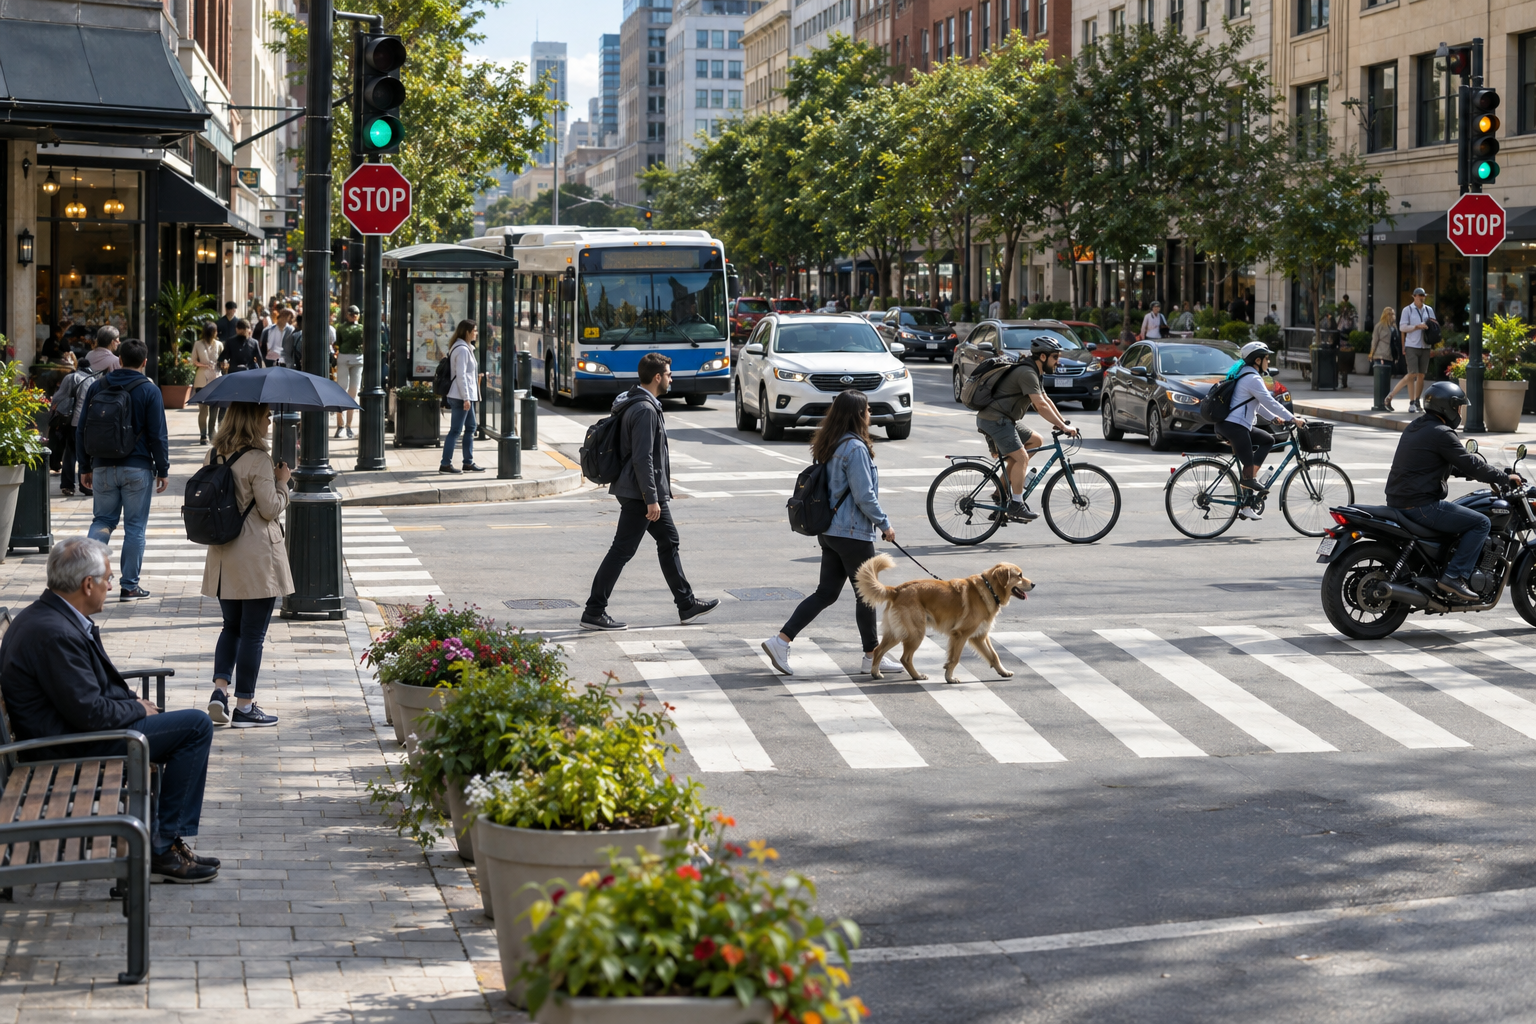
\includegraphics[width=\linewidth]{assets/cnn_busy_street_input.png}\\[1mm]
  \small\textbf{Input:} unannotated 1536-by-1024 street scene
\end{minipage}\hfill
\begin{minipage}[t]{0.485\textwidth}
  \centering
  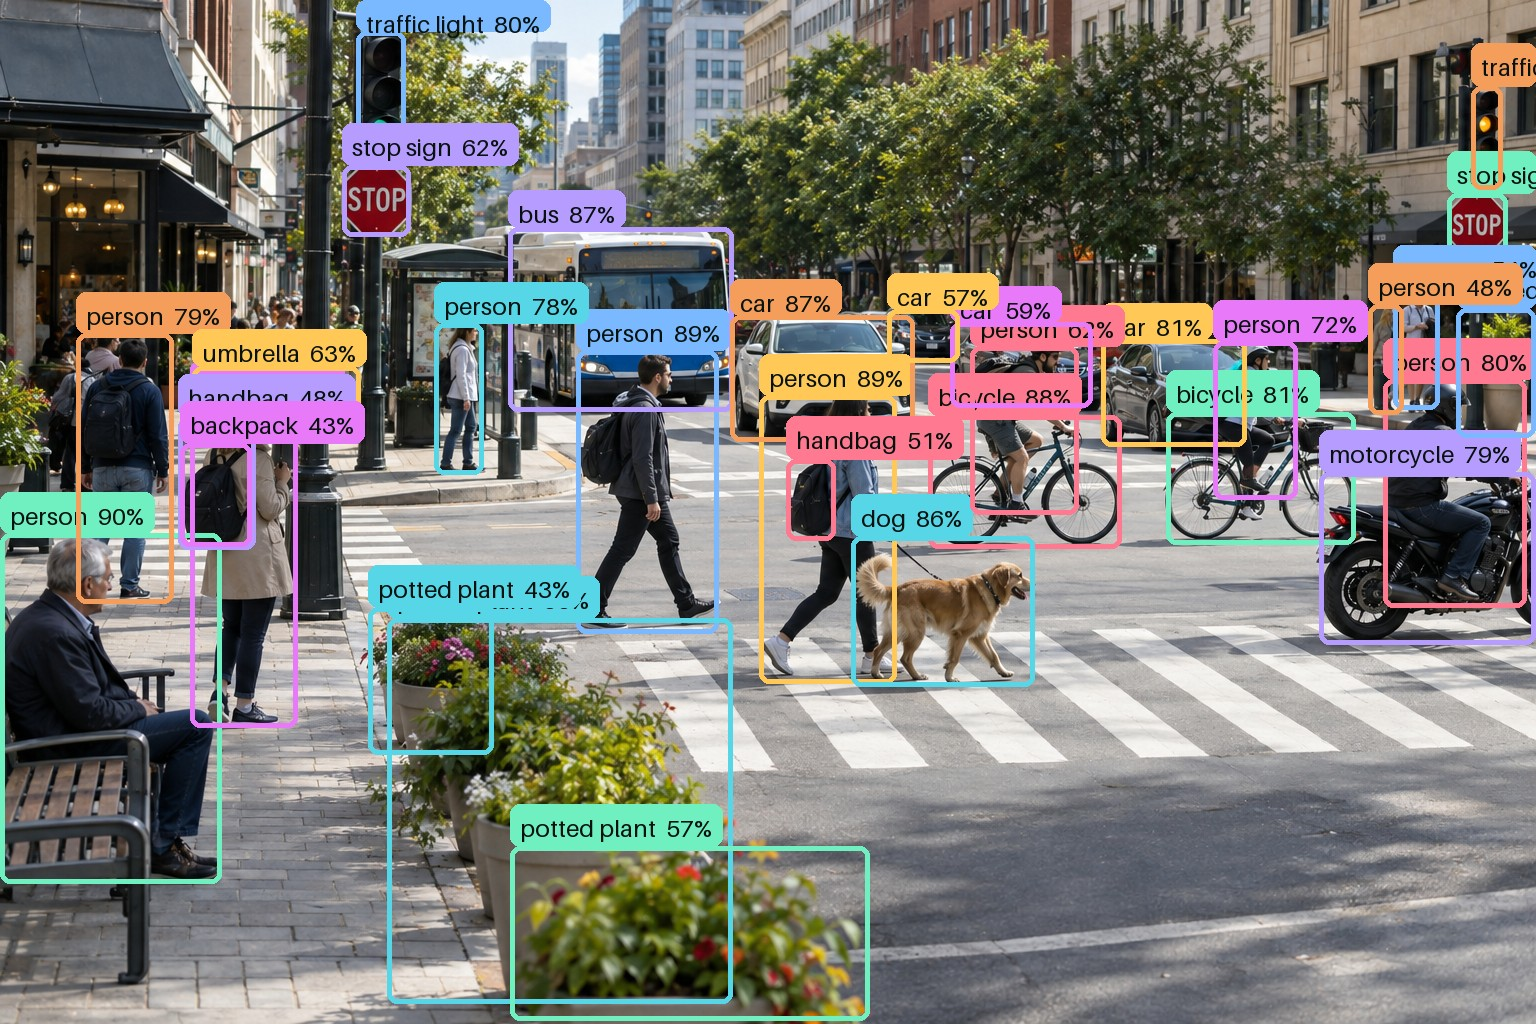
\includegraphics[width=\linewidth]{assets/cnn_05_annotated_busy_street.jpg}\\[1mm]
  \small\textbf{Output:} YOLO boxes, labels, and confidence percentages
\end{minipage}
\caption{Exact CNN experiment before and after website inference. The input
bytes on the left produced the annotated JPEG returned by the Flask API on the
right.}
\label{fig:cnn-before-after}
\end{figure}

\begin{table}[H]
\centering\small
\caption{Observed output for the busy-street CNN experiment.}
\begin{tabularx}{\textwidth}{p{0.24\textwidth}Y}
\toprule
\textbf{Displayed output} & \textbf{Recorded value and meaning} \\
\midrule
Accepted input & PNG street scene, 1536 by 1024 pixels, processed at a 35\% minimum-confidence threshold. \\
Detected boxes & 32 boxes remained after confidence filtering and overlap suppression. \\
Unique classes & 12: person, bicycle, bus, car, dog, traffic light, motorcycle, stop sign, umbrella, potted plant, handbag, and backpack. \\
Strongest examples & Person 90\%, person 89\%, bicycle 88\%, bus 87\%, car 87\%, and dog 86\%. \\
Warm inference time & 88 ms on the capture machine; timing depends on hardware and model warm-up. \\
\bottomrule
\end{tabularx}
\end{table}

\subsection{Choose an input}
After starting \texttt{python app.py}, open the page and choose one of two tabs:
\begin{itemize}
  \item \textbf{Upload photo}: click or drag a JPG, PNG, WEBP, or BMP no larger
  than 12 MB. A preview and filename confirm the selection.
  \item \textbf{Use camera}: allow browser camera permission, aim at the scene,
  and capture a frame. Camera access normally requires localhost or HTTPS.
\end{itemize}
Do not upload private images to a server you do not trust. This local code does
not intentionally save them, but deployment operators remain responsible for
transport security, logs, and retention policy.

\subsection{Run and understand the answer}
Set the confidence slider from 10\% to 90\% (35\% is a useful starting point),
then press \textbf{Detect objects}.
\begin{itemize}
  \item \textbf{Annotated photo}: each colored rectangle is a predicted object
  location. Its tag contains class name and rounded confidence.
  \item \textbf{Detected objects}: a strongest-first list. Matching colors link
  list cards to boxes.
  \item \textbf{Count}: number of boxes surviving the chosen confidence and the
  model's suppression process, not necessarily the true object count.
  \item \textbf{Time}: server inference elapsed milliseconds. It excludes some
  browser/network work and varies by CPU/GPU and first model load.
  \item \textbf{Image size/model/threshold}: records the exact request context.
  \item \textbf{Save result}: downloads the annotated JPEG; reset clears the
  current input and output.
\end{itemize}

If the output says no objects, try a clear, well-lit photo, reduce confidence a
little, or remember that the object may not be one of the 80 known categories.
If the model cannot start, activate the environment, install requirements, and
confirm \texttt{yolov8n.pt} is readable. A 400 error indicates an invalid input;
413 means too large; 503 means the detector could not load/analyze. The first
successful run is normally slower because the model changes from ``cold'' to
``loaded.''

\section{Conclusion}
Sightline joins a pretrained visual learner to a defensive, understandable web
pipeline. The lab distinguishes pixels, learned CNN features, YOLO detections,
application-side validation, and user-facing evidence while making the limits
of confidence and label coverage explicit.

\fi
\chapter*{Overall Conclusion}
\addcontentsline{toc}{chapter}{Overall Conclusion}
\ifdefined\AssignmentVersion
The two assignment problems show learning and probabilistic reasoning from
different directions. The Perceptron changes weights after mistakes until one
line separates suitable labeled points. The HMM keeps its states hidden and
uses emissions, transitions, Viterbi decoding, and posterior probabilities to
explain an observed sequence. Together they emphasize that a model's structure
must match the question: a static boundary and a time-dependent hidden story
are not interchangeable.

Both websites expose the reasoning behind the output. Perceptron users see the
line, weights, errors, and epochs; HMM users see the route, switches, path
probability, and state posterior at each toss. These explanations make the
algorithms testable while preserving the limits of synthetic educational data.
\else
The five laboratory problems cover complementary learning strategies. KNN
consults nearby stored examples; the Decision Tree follows auditable questions;
the SVM learns a wide linear margin; K-Means discovers unlabeled groups; and
CNN/YOLO turns pixels into multiple located object hypotheses. Their websites
expose the evidence most natural to each model: neighbors, a branch path, a
margin, moving centroids, or bounding boxes.

Across all five projects, a model's output inherits the limits of its data and
objective. Synthetic labels can teach mechanics but cannot establish clinical
truth. Training-set accuracy cannot replace independent evaluation, an SVM
score is not automatically a probability, and a cluster is not automatically
meaningful. Keeping those distinctions beside the interactive controls is as
important as implementing the formula.
\fi

\appendix
\chapter{Verification and Reproduction}
\section{Commands verified in this workspace}
The following checks were executed against the submitted sources before this
report was produced.

\begin{longtable}{p{0.24\textwidth}p{0.50\textwidth}p{0.16\textwidth}}
\toprule
\textbf{Project} & \textbf{Verification command} & \textbf{Observed result} \\
\midrule
\endhead
\ifdefined\AssignmentVersion
Perceptron & \texttt{python -m unittest discover -s tests -v} & 12 tests passed \\
HMM & \texttt{python -m unittest discover -s tests -p test\_hmm.py -v}; \texttt{node tests/test\_browser\_hmm.js} & 5 Python tests; browser tests passed \\
\else
KNN & \texttt{python -m unittest discover -s tests -p test\_knn.py -v}; \texttt{node tests/test\_browser\_model.js} & 4 Python tests; browser tests passed \\
Decision Tree & \texttt{python -m unittest discover -s tests -p test\_decision\_tree.py -v}; \texttt{node tests/test\_browser\_tree.js} & 5 Python tests; browser tests passed \\
SVM & \texttt{python -m unittest discover -s tests -p test\_svm.py -v}; \texttt{node tests/test\_browser\_model.js} & 4 Python tests; browser tests passed \\
K-Means & \texttt{node --check dist/app.js} & Syntax check passed \\
CNN/YOLO web layer & \texttt{python -m pytest tests/test\_app.py -q} & 4 tests passed \\
\fi
\bottomrule
\end{longtable}

\ifdefined\AssignmentVersion
The Perceptron checks include exact hard-limit behavior, update equations, API
validation, separable convergence, and bounded non-convergence. The HMM checks
compare the Python and browser-facing calculations for validation, Viterbi, and
forward-backward behavior.
\else
The KNN retraining command reported 60 rows, a 48/12 deterministic split, and
100\% test accuracy. Decision Tree reported 48 rows and 100\% training accuracy.
SVM reported 40 rows and 100\% training accuracy. These values reproduce the
designed laboratory datasets and are not claims of population performance.
\fi

\section{One-page run checklist}
\begin{enumerate}
  \item Install each project's declared dependencies before starting its server.
\ifdefined\AssignmentVersion
  \item For the Perceptron, submit labeled points and watch whether the line
  converges; for HMM, enter only H/T observations and distinguish decoding from
  training.
  \item Serve the HMM \texttt{dist} folder over localhost so its scripts load
  normally.
\else
  \item For KNN, Decision Tree, or SVM, rerun \texttt{python train\_model.py}
  whenever its CSV or training code changes.
  \item Serve browser-only \texttt{dist} folders over localhost so JSON and
  scripts load normally.
\fi
  \item Wait for the page's ready indicator before entering a prediction.
  \item Keep the units printed beside each field and interpret the evidence
  panel together with the main label.
\ifdefined\AssignmentVersion\else
  \item Never use the health demonstrations for diagnosis or urgent decisions.
\fi
\end{enumerate}

\chapter{Glossary for a First-Time Reader}
\begin{longtable}{p{0.23\textwidth}p{0.68\textwidth}}
\toprule
\textbf{Word} & \textbf{Plain meaning in this report} \\
\midrule
\endhead
Algorithm & A precise recipe of steps a computer follows. \\
Feature & An input fact, such as height, glucose, or one pixel value. \\
Target/label & The example answer supplied during supervised learning. \\
\ifdefined\AssignmentVersion
Training & Adjusting a model from examples; the Perceptron trains, while the current HMM page performs inference from user-set probabilities rather than training them. \\
\else
Training & Adjusting or constructing a model from examples; KNN mainly stores its labeled examples, while the other lab models learn parameters, rules, groups, or visual features. \\
\fi
Inference/prediction & Applying an existing model to a new input. \\
\ifdefined\AssignmentVersion
Parameter & A learned or chosen number that affects behavior, such as a Perceptron weight or an HMM transition probability. \\
\else
Parameter & A learned or chosen number that affects behavior, such as a weight, threshold, neighbor count, centroid, or confidence cutoff. \\
\fi
Epoch & One complete pass through all training examples. \\
Accuracy & Fraction of checked labels predicted correctly; its meaning depends completely on which rows were checked. \\
Overfitting & Learning training details so narrowly that new-data performance becomes worse. \\
\ifdefined\AssignmentVersion
Posterior & Probability of a hidden state after considering the complete observation sequence. \\
\else
Standardization & Subtracting a feature's mean and dividing by its standard deviation. \\
Confidence & A model score associated with a guess; it is not a guarantee. \\
Centroid & The coordinate-wise average position of a cluster. \\
\fi
JSON & A text structure of names, arrays, numbers, and objects shared with the browser. \\
API & A defined request/response doorway between pieces of software. \\
\bottomrule
\end{longtable}

\begin{thebibliography}{99}
\addcontentsline{toc}{chapter}{References}

\ifdefined\AssignmentVersion
\bibitem{hagan}
M. T. Hagan, H. B. Demuth, M. H. Beale, and O. De Jes\'{u}s,
\emph{Neural Network Design}, 2nd ed. Stillwater, OK, USA, 2014. [Online].
Available: \url{https://hagan.okstate.edu/nnd.html}

\bibitem{rosenblatt}
F. Rosenblatt, ``The perceptron: A probabilistic model for information storage
and organization in the brain,'' \emph{Psychological Review}, vol. 65, no. 6,
pp. 386--408, 1958, doi: 10.1037/h0042519.

\else
\bibitem{coverhart}
T. Cover and P. Hart, ``Nearest neighbor pattern classification,''
\emph{IEEE Transactions on Information Theory}, vol. 13, no. 1, pp. 21--27,
Jan. 1967, doi: 10.1109/TIT.1967.1053964.

\bibitem{cdcBMI}
Centers for Disease Control and Prevention, ``Adult BMI calculator,'' 2024.
[Online]. Available: \url{https://www.cdc.gov/bmi/adult-calculator/}.
[Accessed: Sep. 13, 2026].

\bibitem{accChestPain}
American College of Cardiology, ``2021 AHA/ACC chest pain guideline,'' Oct.
2021. [Online]. Available:
\url{https://www.acc.org/Guidelines/Guidelines/2021/10/28/12/34/Chest-Pain}.
[Accessed: Sep. 13, 2026].

\bibitem{nhlbiDiagnosis}
National Heart, Lung, and Blood Institute, ``Heart attack diagnosis,'' Mar.
2022. [Online]. Available:
\url{https://www.nhlbi.nih.gov/health/heart-attack/diagnosis}.
[Accessed: Sep. 13, 2026].

\bibitem{breiman}
L. Breiman, J. H. Friedman, R. A. Olshen, and C. J. Stone,
\emph{Classification and Regression Trees}. Belmont, CA, USA: Wadsworth,
1984.

\bibitem{niddk}
National Institute of Diabetes and Digestive and Kidney Diseases, ``Diabetes
tests and diagnosis,'' Dec. 2022. [Online]. Available:
\url{https://www.niddk.nih.gov/health-information/diabetes/overview/tests-diagnosis}.
[Accessed: Sep. 13, 2026].

\bibitem{cortes}
C. Cortes and V. Vapnik, ``Support-vector networks,'' \emph{Machine Learning},
vol. 20, pp. 273--297, 1995, doi: 10.1007/BF00994018.

\bibitem{macqueen}
J. MacQueen, ``Some methods for classification and analysis of multivariate
observations,'' in \emph{Proc. 5th Berkeley Symp. Mathematical Statistics and
Probability}, vol. 1, 1967, pp. 281--297. [Online]. Available:
\url{https://digicoll.lib.berkeley.edu/record/113015?v=pdf}

\fi
\ifdefined\AssignmentVersion
\bibitem{rabiner}
L. R. Rabiner, ``A tutorial on hidden Markov models and selected applications
in speech recognition,'' \emph{Proceedings of the IEEE}, vol. 77, no. 2,
pp. 257--286, Feb. 1989, doi: 10.1109/5.18626.

\else
\bibitem{redmon}
J. Redmon, S. Divvala, R. Girshick, and A. Farhadi, ``You only look once:
Unified, real-time object detection,'' in \emph{Proc. IEEE Conf. Computer
Vision and Pattern Recognition}, 2016, pp. 779--788. [Online]. Available:
\url{https://openaccess.thecvf.com/content_cvpr_2016/html/Redmon_You_Only_Look_CVPR_2016_paper.html}

\bibitem{ultralyticsV8}
Ultralytics, ``Ultralytics YOLOv8,'' [Online]. Available:
\url{https://docs.ultralytics.com/models/yolov8/}. [Accessed: Sep. 13, 2026].

\bibitem{coco}
T.-Y. Lin \emph{et al.}, ``Microsoft COCO: Common objects in context,'' in
\emph{Computer Vision--ECCV 2014}, 2014, pp. 740--755,
doi: 10.1007/978-3-319-10602-1\_48.

\bibitem{flaskUpload}
Pallets, ``Uploading files,'' \emph{Flask Documentation}. [Online]. Available:
\url{https://flask.palletsprojects.com/en/stable/patterns/fileuploads/}.
[Accessed: Sep. 13, 2026].

\bibitem{pillow}
Pillow Contributors, ``Pillow documentation,'' [Online]. Available:
\url{https://pillow.readthedocs.io/}. [Accessed: Sep. 13, 2026].

\bibitem{ultralyticsTrain}
Ultralytics, ``Train mode,'' \emph{Ultralytics YOLO Documentation}. [Online].
Available: \url{https://docs.ultralytics.com/modes/train/}.
[Accessed: Sep. 13, 2026].

\fi
\end{thebibliography}

\end{document}
